\documentclass[sigconf]{acmart}

% Remove this for camera-ready
\settopmatter{printacmref=false} % Removes citation information below abstract
\renewcommand\footnotetextcopyrightpermission[1]{} % removes footnote with conference information in first column
\settopmatter{printfolios=true}

\usepackage{times}
\usepackage[utf8]{inputenc}
\usepackage{url}
\usepackage{array,multirow}
\usepackage{xspace}
\usepackage{xcolor}
\usepackage{color, colortbl} 
\usepackage{balance}
\usepackage{paralist}
\usepackage{cleveref}
%\usepackage{amssymb}
\usepackage{graphicx}
\usepackage{pifont}
\usepackage{array}
\usepackage{booktabs}
\usepackage{tikz}
\usepackage{bm}
\usepackage{enumitem}
\setlength {\marginparwidth}{2cm}
\usepackage{todonotes}
\usepackage{arydshln}
\usepackage{makecell}
\usepackage{tabularx}
\usepackage{authblk}
\usepackage{caption}
\usepackage{soul,color}
%\usepackage{subcaption}
\usepackage{mwe}
\usepackage{ifthen}
\usepackage{algorithm}
\usepackage[noend]{algpseudocode}
\usepackage{epsfig}
\usepackage[tight,footnotesize]{subfigure}

\newcommand{\cmark}{\ding{51}}%
\newcommand{\xmark}{\ding{55}}%

%!TEX root = main.tex
%=========================================================

% use true/false to toggle all comments (both kinds)

\newboolean{showcomments}
\setboolean{showcomments}{true}

% ====== comments ======
\newcommand\important[1]{\todo[inline]{\textbf{Important:} #1}}
\newcommand\alberto[1]{\todo[color=yellow,inline]{\textbf{Alberto:} #1}}
\newcommand\etienne[1]{\todo[color=orange,inline]{\textbf{Etienne:} #1}}
\newcommand\pierre[1]{\todo[color=brown,inline]{\textbf{Pierre:} #1}}
\newcommand\felix[1]{\todo[color=blue!40,inline]{\textbf{Felix:} #1}}
\newcommand\michal[1]{\todo[color=green,inline]{\textbf{Michał:} #1}}
\newcommand\onur[1]{\todo[color=red,inline]{\textbf{Onur:} #1}}
\newcommand\sergi[1]{\todo[color=pink,inline]{\textbf{Sergi:} #1}}
\newcommand\ramin[1]{\todo[color=brown,inline]{\textbf{Ramin:} #1}}
\newcommand\mustafa[1]{\todo[color=brown,inline]{\textbf{Mustafa:} #1}}
% Uncomment the following command to make all comments disappear
\ifthenelse{\boolean{showcomments}} { }
{
\renewcommand\important[1]{}
\renewcommand\alberto[1]{}
\renewcommand\mustafa[1]{}
\renewcommand\michal[1]{}
\renewcommand\onur[1]{}
\renewcommand\sergi[1]{}
\renewcommand\etienne[1]{}
\renewcommand\pierre[1]{}
\renewcommand\ramin[1]{}
}

% ====== inlined and toggable comments ======

\ifthenelse{\boolean{showcomments}}
{ \newcommand{\mynote}[3]{
    \protect\fbox{\bfseries\sffamily\scriptsize#1}
    {\small\textsf{\emph{\color{#3}{#2}}}}}}
{ \newcommand{\mynote}[3]{}}

\newcommand{\er}[1]{\mynote{Etienne}{#1}{blue}}
\newcommand{\mk}[1]{\mynote{Michał}{#1}{brown}}
\newcommand{\sr}[1]{\mynote{Sergi}{#1}{red}}

% \newcommand{\xxx}[1]{\mynote{YourName}{#1}{black!20!red!80!}}
% \newcommand{\xxx}[1]{\mynote{YourName}{#1}{green}}
\newcommand{\as}[1]{\mynote{Alberto}{#1}{orange}}
\newcommand{\dk}[1]{\mynote{Daniel}{#1}{green}}
\newcommand{\rs}[1]{\mynote{Ramin}{#1}{violet}}
\newcommand{\oa}[1]{\mynote{Onur}{#1}{red}}

% ====== systems ======
\newcommand\sysname{TOPDISC\xspace}
\newcommand\altname{DHT\xspace}
\newcommand\altsysname{PMETIS\xspace}
\newcommand\sysnamePriv{Pineapple\xspace}
\newcommand\sysnameAnon{\coconut}
\newcommand\libcoin{LibraCoin\xspace}
\newcommand\libcoins{LibraCoins\xspace}
\newcommand\privcoin{PrivCoin\xspace}
\newcommand\privcoins{PrivCoins\xspace}

\newcommand\sysnamereplay{\texttt{byzcuit}\xspace}
\newcommand\sysnamebaseline{\texttt{byzcuit-baseline}\xspace}
\newcommand\simplesysname{Simple-\sysname}

\newcommand\libra{Libra\xspace}
\newcommand\fourier{Fourier\xspace}
\newcommand\chainspace{Chainspace\xspace}
\newcommand\ethereum{Ethereum\xspace}
\newcommand\hyperledger{Hyperledger\xspace}
\newcommand\omniledger{Omniledger\xspace}
\newcommand\rapidchain{RapidChain\xspace}
\newcommand\elgamal{El-Gamal\xspace}
\newcommand\coconut{Coconut\xspace}
\newcommand\macggm{$\bm{\mathrm{MAC_{GGM}}}$\xspace}
\newcommand\sbac{S-BAC\xspace}
\newcommand\bft{BFT\xspace}
\newcommand\atomix{Atomix\xspace}
\newcommand\cscoin{CSCoin\xspace}
\newcommand\rscoin{RSCoin\xspace}
\newcommand\lsbac{\sysname}
\newcommand\fsbac{F-SBAC\xspace}
\newcommand\bftsmart{\textsc{bft-SMaRt}\xspace}

\makeatletter
\def\BState{\State\hskip-\ALG@thistlm}
\makeatother

% ====== custom notations ======
%\newcommand\algorithm[1]{\textsf{#1}}
\newcommand\hashtopoint{H^*\xspace}
\newcommand\stringtopoint{H'\xspace}
\newcommand\function[1]{\ding{118}\xspace \textsf{#1}:\xspace}
\newcommand\shard[1]{\emph{shard}\xspace#1\xspace}
\newcommand\Shard[1]{\emph{Shard}\xspace#1\xspace}
\newcommand\preacceptt{\textsf{pre-accept}($T$)\xspace}
\newcommand\preabortt{\textsf{pre-abort}($T$)\xspace}
\newcommand\preaccepttt{\textsf{pre-accept}($T'$)\xspace}
\newcommand\preaborttt{\textsf{pre-abort}($T'$)\xspace}
\newcommand\preacceptttt{\textsf{pre-accept}($T''$)\xspace}
\newcommand\preacceptts{\textsf{pre-accept}($T,s_T$)\xspace}
\newcommand\preabortts{\textsf{pre-abort}($T,s_T$)\xspace}
\newcommand\preabortttt{\textsf{pre-abort}($T''$)\xspace}
\newcommand\acceptt{\textsf{accept}($T$)\xspace}
\newcommand\abortt{\textsf{abort}($T$)\xspace}
\newcommand\accepttt{\textsf{accept}($T'$)\xspace}
\newcommand\aborttt{\textsf{abort}($T'$)\xspace}
\newcommand\acceptttt{\textsf{accept}($T''$)\xspace}
\newcommand\abortttt{\textsf{abort}($T''$)\xspace}
\newcommand\acceptts{\textsf{accept}($T,s_T$)\xspace}
\newcommand\abortts{\textsf{abort}($T,s_T$)\xspace}
\newcommand\myrow[1]{row\xspace\textsf{#1}\xspace}
\newcommand\mycolumn[1]{column\xspace\textsf{#1}\xspace}
\newcommand\shardled{shard-led\xspace}
\newcommand\Shardled{Shard-led\xspace}
\newcommand\clientled{client-led\xspace}
\newcommand\Clientled{Client-led\xspace}
\newcommand\activeObj{`active'\xspace}
\newcommand\inactiveObj{`inactive'\xspace}
\newcommand\locked{`locked'\xspace}
\newcommand\wa{{WA}\xspace}
\newcommand\wb{{WB}\xspace}
\newcommand\ka{{KA}\xspace}
\newcommand\kb{{KB}\xspace}

% ====== concepts/terminology =======

\newcommand\attacker{attacker\xspace}
\newcommand\adversary{attacker\xspace}
\newcommand\prerecorded{prerecorded\xspace}
\newcommand\prerecords{prerecords\xspace}
\newcommand\prerecord{prerecord\xspace}

%  ===== formatting ======
% Abbreviations etc.
\newcommand{\cf}{cf.\@\xspace}
\newcommand{\vs}{vs.\@\xspace}
\newcommand{\etc}{etc.\@\xspace}
\newcommand{\ala}{ala\@\xspace}
\newcommand{\wrt}{w.r.t.\@\xspace}
\newcommand{\etal}{\textit{et al.}\@\xspace}
\newcommand{\eg}{\textit{e.g.}\@\xspace}
\newcommand{\Eg}{\textit{E.g.}\@\xspace}
\newcommand{\ie}{\textit{i.e.}\@\xspace}
\newcommand{\Ie}{\textit{I.e.}\@\xspace}
\newcommand{\via}{\textit{via}\@\xspace}
\newcommand{\defacto}{\textit{de facto}\@\xspace}

\newcommand\mypara[1]{\vspace{0.05in} \noindent \textbf{#1.}}
\newcommand\para[1]{\vspace{0.05in} \noindent \textbf{#1.}}


\newcommand\definition[2]{\ding{118}\xspace \textsf{#1}\xspace$\bm{\rightarrow}$\xspace(#2):\xspace}



% For inlined section titles.
\newcommand\inlinesection[1]{{\bf #1.}}

\def\first{({\it i})\xspace}
\def\second{({\it ii})\xspace}
\def\third{({\it iii})\xspace}
\def\fourth{({\it iv})\xspace}
\def\fifth{({\it v})\xspace}
\def\sixth{({\it vi})\xspace}

\newcommand{\one}{({\em i})\xspace}
\newcommand{\two}{({\em ii})\xspace}
\newcommand{\three}{({\em iii})\xspace}
\newcommand{\four}{({\em iv})\xspace}
\newcommand{\five}{({\em v})\xspace}

% Colours
\definecolor{verylightgray}{gray}{0.8}

% Table
\newcolumntype{L}{l<{\hspace{1cm}}}
\newcolumntype{C}{c<{\hspace{1cm}}}
\newcolumntype{D}{c<{\hspace{0.3cm}}}

% Markers
\newcommand\vgap{\vskip 2ex}
\newcommand\marker{\vgap\ding{118}\xspace}

\def\na{--}
\def\unsure{?}
\def\missing{$!$}
\newcommand{\yes}{\ding{51}}
\newcommand{\no}{\ding{55}}
\DeclareRobustCommand\pie[1]{
\tikz[every node/.style={inner sep=0,outer sep=0, scale=1.5}]{
\node[minimum size=1.5ex] at (0,-1.5ex) {}; 
 \draw[fill=white] (0,-1.5ex) circle (0.75ex); \draw[fill=black] (0.75ex,-1.5ex) arc (0:#1:0.75ex); 
}
}
\def\L{\pie{0}} % Low
\def\M{\pie{-180}} % Medium
\def\H{\pie{360}} % High


\begin{document}

\title{Topic-based service discovery for the Ethereum P2P network}
\author{}


\begin{abstract}
Peer-to-Peer (P2P) Networks  are being increasingly deployed in distributed systems. They are being used in blockchains (Ethereum, Bitcoin), storage systems (IPFS, Stor4j) and more. One of the main functionality of P2P network is the ability to collectively keep information in the form of a key-value store. However, the current implementations either trade security for efficiency (structured P2P networks) or vice-versa (unstructured P2P networks). 

In this work, we propose \sysname - a P2P key/value store implementation which enables secure, efficient and robust information storage and retrieval. Our system can be deployed on any Distributed Hash Table (DHT). \sysname stores data on multiple nodes for increased security that can be later found within abounded amount of time guaranteeing high efficiency. We implement a robust admission mechanism limiting the resource usage by its participants and preventing a vast range of malicious behaviours. 

We present the design of \sysname and evaluate the system in multiple scenarios. Compared to the state-of-the-art, our system achieves high security, more equal load distribution, lower computational and communication overhead and better robustness in the presence of a powerful attacker.

%The Ethereum blockchain runs a Peer-to-Peer (P2P) network that rely on Kademlia Distributed Hash Table (DHT) for peer discovery and exchanging pending transactions and mined blocks. 
%Apart from supporting blockchain data exchange, the Ethereum P2P network is used by other applications taking advantage of the existing infrastructure to facilitate bootstraping of their own, application-specific networks. However, in order to achieve this task, peers using the same application must first find each other among other, unrelated nodes.

%In this work, we propose a service discovery system (\sysname) which enables secure and robust discovery of application-specific peers in a large, host P2P network. 
%Our system enables nodes to associate themselves with a set of \emph{topics}. The association is collectively stored by the network, and can be later found by interested peers within a bounded amount of time. \sysname included a robust admission mechanism limiting the resource usage by its participants and preventing a vast range of malicious behaviours. 

%We present the design of \sysname and evaluate the system in multiple scenarios. Compared to the state-of-the-art, our system achieves more equal load distribution, lower computational and communication overhead and better robustness in the presence of a powerful attacker.
\end{abstract}

\maketitle
%%!TEX root = ../main.tex
%=========================================================

\section{Introduction}
\para{Motivation} Ethereum~\cite{buterin2013ethereum}  is one of the largest permissionless,  open-source  blockchains supporting Turing-complete scripting via smart contracts. Ethereum runs a Peer-to-Peer (P2P) network based on Kademlia Distributed Hash Table (DHT) ~\cite{maymounkov2002kademlia} to exchange pending transactions and mined blocks. 

%Following its decentralized design, Ethereum relies on a Peer-to-Peer (P2P) communication network, where individual nodes, running an Ethereum client software (\eg Go Ethereum~\cite{go-ethereum}), send and receive messages containing transactions and blocks to achieve distributed consensus, without relying on any central node or a trusted third party. The core system and the associated protocols used by the peers to participate in the Ethereum P2P network is included as part of a suite called DEVp2p. The suite includes individual sub-systems and protocols for services such as node discovery or establishing secure or point-to-point communication between peers. 

Apart from supporting blockchain data exchange, the Ethereum P2P network is also used by other applications. This includes multiple Ethereum testnets (Ropsten, Rinkeby),  alternative cryptocurrencies(Pirl, Musicoin) and other decentralized platforms such as iExec or Swarm.
In 2018, the Ethereum P2P network nodes operated a total of 4,076 different applications\cite{kim2018measuring}. Most of those applications require a dedicated P2P network to disseminate application-specific messages (\eg event notifications) to the interested peers but rely on the larger, Ethereum P2P network for bootstrapping.

Using an existing, well-established P2P network to bootstrap smaller, application specific networks has multiple advantages. Firstly, it encourages re-using reliable code to perform common tasks such as securing connections or finding peers. Secondly, P2P network security increases with the number of its honest participants. Being part of a larger swarm makes smaller applications more resistant to various attacks\hl{some refs from attack of smaller blockchains}. Finally, application developers can focus uniquely on implementing application-specific services boosting the growth of the entire, decentralised ecosystem. 

To realise this vision, nodes must \textit{(i)} join a larger, host P2P network, \textit{(ii)} discover their application-specific peers, \textit{(iii)} form an application-specific network. However, peer discovery in a fully decentralised setup is a challenging task. Unlike existing discovery protocols that work in a local setting (MDNS/Bonjour\hl{[?]}) or rely on trusted operators \hl{[?]}, decentralised node discovery must work at a global scale and in a fully decentralised setting. Due to the high heterogeneity of applications and (potentially constraint) peers, such a protocol must be efficient and introduce low communication and computational overhead. Finally, an open system, must protect against malicious actors trying to disturb network services, exhaust resources of honest peers or hijack application-specific networks. 

\para{State of the art} In the current Ethereum service discovery system, \ie discovery version 4 (Discv4), nodes perform a \textit{brute-force} discovery process. A node willing to discover application-specific peers randomly traverses the DHT and initiates connections with all the encountered nodes. A permanent connection is established only if a peer supports the same application and terminated otherwise. Such an approach provides strong security guarantees but results in a large communication overhead and long discovery times, particularly for unpopular applications with a small number of peers. While multiple, alternative discovery systems have been proposed \hl{[?]}, they rely on unrealistic assumptions \hl{[?]}, introduce high overhead or fail to operate in a presence of an adversary \hl{[?]}. 

\para{Discv5} In this work, we propose the discovery system version 5 (\textit{\sysname}) --- a \textbf{service discovery protocol} which enables secure, efficient and robust discovery of application-specific peers. Different from Discv4, \sysname allows nodes (\ie advertisers) to associate themselves with a set of \emph{topics} (\eg application IDs), and advertise the association (\ie an ad) to the network. The information is collectively stored by network participants (\ie registrars) without relying on a single trusted party at any point. Any node can then query the network for a topic to obtain a list of application-specific peers and directly connect to them without disturbing other members of the network. 

We build \sysname on top of the existing Ethereum DHT to avoid major changes to the system and take advantage of the already existing routing infrastructure. The protocol propagates application-specific advertisements to multiple nodes chosen in an unpredictable way to protect against targeted attacks. Our design encourages diversity of advertisements stored at each registrar making the system resistant to network dynamics. At the same time, \sysname provides efficient peer discovery operations terminating within a bounded number of steps for all the topics regardless of their popularity. The protocol implements a robust admission mechanism to limit the resource usage on all the nodes, ensure fairness across topics, and prevent a vast range of malicious behaviours even in the presence of a powerful attacker.

\para{Contributions} We make the following contributions:
\begin{itemize}
    \item In \Cref{sec:placement}, we design a DHT-based data placement system that distributes service advertisement in the network. The protocol combines pseudo-random data placement for security with deterministic operations for efficiency. We present a lookup operation that finds a subset of advertisement placed in the system within a bounded amount of time. The procedure ensure the diversity of data sources and is resistant against manipulation by malicious registrars. 
    \item In \Cref{sec:registration} we design a lightweight admission protocol allowing advertisers to place ads after waiting for a specified amount of time. \sysname guarantees that advertisers cannot place more advertisement by deviating from the protocol and does not create any intermediary state at nodes holding the advertisements. 
    \item In \Cref{sec:waitingTime}, we design a function that calculates a waiting time after which advertisement can be placed on nodes holding advertisements. The function limits the amount of resources used by each node, promotes ads diversity stored within nodes, and protects against a vast range of malicious behaviours. 
\end{itemize}

In \Cref{sec:eval}, we evaluate \sysname under different system parameters and against state-of-the-art decentralised discovery systems. Our system achieves better load-balancing and requires more resource consumption by the attackers to successfully launch attacks such as eclipsing attacks. We also provide performance evaluation results from both simulations and from real system deployment. \sysname is scheduled for implementation in the next version of the Ethereum P2P network. 

%\michal{From the paragraph below we should form a requirements parts}
% An open and decentralized discovery system introduces new security challenges that need to be addressed. Malicious nodes may decide to deviate from the protocol in order to increase their own visibility or disrupt system operations. A particularly important security challenge is the \textit{Sybil attack} which can amplify the attacking power of malicious nodes, typically with very little resource consumption. The Sybils can launch various attacks including Denial-of-Service (DoS) by ignoring ad lookups, spam ads with bogus topic advertisement, and launch more sophisticated attacks to isolate nodes from their peers in their target sub-networks (\ie eclipse attack). 
%\michal{The above needs completion}
%\ramin{Is the above information about attacks needed in the introduction?}
%\michal{Probably not. We must just say there are problems with security}




%!TEX root = ../main.tex
%=========================================================

\section{Introduction}
Ethereum~\cite{buterin2013ethereum}  is one of the largest permission-less (\ie open membership),  open-source  blockchains supporting Turing-complete scripting via smart contracts. 

In addition to running its own blockchain platform, Ethereum is home to third-party decentralised applications and platforms that run alternative cryptocurrencies and host various services such as content delivery. 

A vast majority of these applications require dedicated ``sub-networks'', each consisting of only the peers participating in a particular application, to enable exchange of application-specific data such as transactions, blocks, \etc to be disseminated to only the peers interested in that data. 

In order to form application-specific sub-networks, the peers must first join an (application-agnostic) Ethereum network and participate in a \textit{service discovery protocol (Discv4)} to find other live peers that are part of the desired application's sub-network. 

The Ethereum network is based on Kademlia\cite{maymounkov2002kademlia} – a well-established Distributed Hash Table (DHT) implementation. 

Unlike the earlier DHT systems, Kademlia follows a flexible peer selection process that allows random sampling of peers from each distance-specific interval along the circle (where identifiers are arranged). 

Each node establishes \textit{DHT-level network connections} with a fixed number of sampled peers from each distance and also adds those peers to the corresponding (distance-specific) entry in its local routing table.

\para{State-of-the-art} Discv4 is the current \textit{service discovery mechanism} of Ethereum. Discv4 merely makes random walks (picking random destinations from the DHT id space) and forms a random sample of peers learned from \textit{encountered nodes} along the walks. 

These sample of peers are then returned to the application, which must determine each peer's supported application, \ie by initiating a handshake protocol with each peer to query their supported applications. 

Until an application forms enough application-level connections with peers of the corresponding application, it requests more peers from Discv4 to continue the \textit{exhaustive search process}.  

The randomness in the sampling of peers in both the DHT-level connections by Kademlia and application-level connections by Discv4 provides (a best-effort) Byzantine resilience in a permission-less network where financially-motivated attacks targeting individual applications are common. 

These application-level attacks use as a precursor the more basic, targeted attacks such as eclipsing where an attacker aims to fill up a peer's application-level connections with its Sybils - afterwards, an application can be fed with any custom data as part of an attack such as double-spending, stubborn mining, \etc. 

In addition to security, another major challenge facing Discv4 is the \textit{scalability}: although random peer selection provides an acceptable-level of security against eclipsing attacks, the current discovery process is rather slow in finding peers for even moderately popular applications. 

As more peers and applications join the Ethereum network, the inefficiency of brute-force discovery process is likely to become a bottleneck for the applications. 

\para{Discv5} In this work, we propose a new \textbf{service discovery layer} which enables secure,  efficient and robust  discovery of application-specific peers in the Ethereum network.
Different from Discv4, \sysname allows nodes (\ie advertisers) to associate themselves with a set of \emph{topics} (\eg application IDs), and advertise the association (\ie an ad) in the network. 

The information is collectively stored by network participants (\ie registrars) without relying on a single trusted party at any point. Any node can then query the network for a topic to obtain a list of application-specific peers and directly connect to them without disturbing other members of the network. 

We build \sysname on top of the existing Kademlia DHT to propagate application-specific advertisements to randomly-sampled nodes chosen in a way for resilience against targeted attacks. 

% Didn't touch the text below
Our design encourages diversity of advertisements stored at each registrar making the system resistant to network dynamics. At the same time, \sysname provides efficient peer discovery operations terminating within a bounded number of steps for all the topics regardless of their popularity. The protocol implements a robust admission mechanism to limit the resource usage on all the nodes, ensure fairness across topics, and prevent a vast range of malicious behaviours even in the presence of a powerful attacker.

\para{Contributions} We make the following contributions:
\begin{itemize}
    \item In \Cref{sec:placement}, we design a DHT-based data placement system that distributes service advertisement in the network. The protocol combines pseudo-random data placement for security with deterministic operations for efficiency. We present a lookup operation that finds a subset of advertisement placed in the system within a bounded amount of time. The procedure ensure the diversity of data sources and is resistant against manipulation by malicious registrars. 
    \item In \Cref{sec:registration} we design a lightweight admission protocol allowing advertisers to place ads after waiting for a specified amount of time. \sysname guarantees that advertisers cannot place more advertisement by deviating from the protocol and does not create any intermediary state at nodes holding the advertisements. 
    \item In \Cref{sec:waitingTime}, we design a function that calculates a waiting time after which advertisement can be placed on nodes holding advertisements. The function limits the amount of resources used by each node, promotes ads diversity stored within nodes, and protects against a vast range of malicious behaviours. 
\end{itemize}



%%!TEX root = ../main.tex
%=========================================================

\section{Background}
\label{sec:background}

\michal{Need a good introduction on Kademlia here. Distances/buckets etc. It's required to explain the ticket table, routing etc.}
\etienne{How different is the Ethereum Kademlia from the original published version? I can assume there have been changes in so many years. Is there a reference document for the Ethereum's Kademlia I can read?}
\sergi{From what i remember main difference are num of buckets and use of log distance.  I don't remember any document but Felix will help.}
\sergi{We should also add how kademlia is used for discovery (when lookups are performed, lookup buffer use,  pool of connections, random lookups, etc}

\subsection{Ethereum DHT}
\michal{Borrowed from \href{https://arxiv.org/pdf/1908.10141.pdf}{this paper}}
Ethereum DHT is based on Kademlia - a UDP-based, peer-to-peer distributed hash table (DHT) that is used to locate data stord in a decentralized way~\cite{maymounkov2002kademlia}. Each node is uniquely identified by its randomly generated node ID. A node ID in Ethereum is a marshaled version of node's public key. It is easy to generate many different identities but computationally infeasible to generate a specific one. A data item stored in the DHT is also found by its key, which is simply a hash of the data itself. Node IDs and data keys share the same representation; in the following we use the term ID for both.
Ethereum DHT stores data at nodes whose node ID is the “closest” to the data’s key. Closeness is defined as the bitwise XOR between two IDs, taken as an integer value, i.e.,$d(x, y) = \textit{log}_2 \lfloor x \oplus y \rfloor$.


A DHT node stores its known peers in a routing table divided into buckets which partition the known network based on the local node’s ID (\Cref{fig:kademlia}). Every bucket stores up to $k$ neighbors. Bucket $i$ stores nodes whose distance is in $[2i, 2i+1)$, which effectively corresponds to the length of the common prefix between two node IDs. The routing table stores a detailed view of peers close to the node and a less detailed view of parts of the network located further away.

Items in the DHT and nodes on the network are located by \emph{lookups}. A lookup successively queries nodes that are closest to the desired target ID (key or node ID). Intuitively, a peer closer to the target ID maintains a more detailed view of the target part of the network and provides the initial node with additional peers to query. For instance, the green node in \Cref{fig:kademlia} looking data ID in \emph{bucket 1} will ask known peers in \emph{bucket 1} that will provide additional peers closer to the data ID. Storing data follow the same process.  

\begin{figure}
    
\includegraphics[width=0.4\textwidth]{img/kademlia}
    \caption{Ethereum DHT routing table.}
    \label{fig:kademlia}
 \end{figure}


\section{Background}
\label{sec:background}
In this section, we provide background on structured and unstructured Peer-to-peer networks. 

\subsection{Peer-to-Peer Networks}
Peer-to-peer (P2P) networks are distributed application architectures that partition tasks or workloads between peers. Peers are equally privileged participants in the application, making P2P networks a sound basis for the decentralised applications. Peers make a portion of their resources, such as processing power, disk storage or network bandwidth, directly available to other network participants, without the need for central coordination by servers or stable hosts. Peers are both suppliers and consumers of resources, in contrast to the traditional client–server model.
% in which the consumption and supply of resources is divided.

P2P networks implement a virtual overlay network on top of the physical network topology, where the nodes in the overlay form a subset of the nodes in the physical network. Data is still exchanged directly over the underlying TCP/IP network, but at the application layer peers are able to communicate with each other directly, via the logical overlay links. Overlays are used for indexing and peer discovery, and make the P2P systems independent from the physical network topology. The two main types of P2P networks are \textit{(i)} unstructured and \textit{(ii)} structured. 

\para{Unstructured P2P Networks}
Unstructured P2P networks do not impose a particular structure on the overlay network by design, but rather are formed by nodes that randomly form connections to each other~\cite{gnutella, gossip, kazaa}. Without a globally imposed structure, unstructured networks are easy to build and are highly robust in the face of high rates of churn. 

On the other hand finding content is difficult in an unstructured network. In the earlier P2P networks such as Gnutella~\cite{gnutella}, the search queries were flooded through the network to find as many peers as possible that share the data. However, flooding is unscalable as its overhead on the network grows linearly with number of search queries, which in turn grows with system size. Furthermore, since there is no correlation between a peer and the content managed by it, there is no guarantee that scoped flooding will find a peer that has the desired data. The problem gets more severe for unpopular content that, while being present only on a few nodes, might be difficult to find. More recent P2P systems use more scalable search mechanisms such as random walk, as we discuss in Section~\ref{P2PsearchEngines}. 


\para{Structured P2P Networks}
In structured P2P networks the overlay is organized into a specific topology, and the protocol ensures that any node can efficiently search the network for content, even if the resource is extremely rare. The most common type of structured P2P networks implement a distributed hash table (DHT)~\cite{kademlia, chord, pastry, can, tapestry} in which a variant of consistent hashing is used to assign responsibility for maintaining each content or resource to a particular peer. This enables peers to search for resources on the network using a hash table; that is, (key, value) pairs are stored in the DHT, and any participating node can efficiently retrieve the value associated with a given key within a bounded number of steps (usually $O(log(n))$, where $n$ is the number of peers in the network).

Unfortunately, maintaining a structured overlay topology makes this type of networks less robust in networks with a high rate of churn. It exposes the network to vast range of attacks that are much more difficult to perform in an unstructured P2P network~\cite{Trifa2012TaxonomyOS}.

\para{P2P Networks in use}
Modern decentralized application usually implement a mix of both types of networks. Ethereum uses a Kademlia DHT traversal to find peers with which it will form an unstructured network used for blocks dissemination. Similarly, IPFS~\cite{ipfs} maintains parallel unstructured (BitSwap) and structured (Kademlia DHT) networks for to store information about location of files stored in the networks. 


%!TEX root = ../main.tex
%=========================================================

\section{System model}
We assume a network of nodes all being part of the Ethereum DHT\footnote{Currently, Ethereum DHT consist of 3,500-5,000 nodes.}. During the bootstrap process, nodes generate public/secret key pairs that are used to secure point-to-point communication with their peers (providing integrity and confidentiality). Each node is identified by its \emph{ID} (hash of the public key) and its IP address. We assume that multiple nodes may share the same IP address (due to NAT or being hosted by the same physical machine). However, no two nodes share the same ID. Nodes can play the following roles:
\begin{itemize}
    \item \textbf{Registrar} - a node that accepts registrations made by advertisers and respond to topic queries. When asked for a specific topic, a registrar should respond with advertisers that registered for the topic the registrar is aware of. All the DHT nodes play this role. Importantly, registrar may hold advertisements for multiple topics. 
    \item \textbf{Advertiser} - nodes that register for a specific topic and want to be discovered by their peers. The advertisers make themselves discoverable by placing advertisements on registrars. Nodes play a topic-specific advertiser role for every topic application it runs.
    \item \textbf{Searcher} - a node that tries to discover advertisers under a specific topic. Nodes play a topic-specific searcher role for every topic application it runs.
\end{itemize}
Multiple advertisers/searchers hosted by the same DHT node will share the same ID and IP address but will differ in topic. 

Our system indexes participants by their registered topic identifiers or topic(s), for short. A \emph{topic} is an identifier for a service provided by a node. A node providing a certain service, each identified with a topic, is said to \emph{place an ad} for itself when it registers the ad on a registrar to make itself discoverable under that topic. An \emph{ad} (\ie advertisement) is the registration of an advertiser for a topic on another node. Depending on the needs of the application, a node can advertise multiple topics or no topics at all. We assuem that the popularity of the topics in the system may vary significantly and follows a power law distribution. 

We assume the presence of malicious nodes in the DHT. The malicious nodes can freely deviate from the protocol and communicate with any other nodes in the network. The malicious node may spawn multiple virtual nodes within one physical machine and thus create multiple IDs. As creating a node requires maintaining periodic, encrypted communication with its peers, the number of active IDs an attacker can posses at a time is limited. We also assume that the number of IP addresses under the control of an attacker is limited. However, an attacker is able to generate more similar IP addresses (within a single subnet) than diverse IP addresses (with different prefixes). We use the number of IP addresses and IDs under the control of an attacker as parameters for our evaluation (\Cref{sec:evaluation}). Regardless of the number of the attacker, we assume that no honest node is fully eclipsed by the malicious ones. \textit{I.e.,} each honest DHT node has at least one honest peer. 


\section{Objectives}
\label{sec:objectives}

In this section, we discuss the objectives of \sysname design and describe the challenges involved in achieving them. A comprehensive list of objectives are listed in \Cref{tab:objectives}, and we discuss them under four main categories: security, fairness, load-balancing, and efficiency of the discovery system. 

\para{Security and Fairness} As an open, decentralised system, \sysname must operate securely under a Byzantine environment where adversaries can generate Sybils at no cost and launch various attacks on \sysname to disrupt discovery of and to eclipse peers of target applications (\textbf{G8}). Eclipsing is often a precursor to application-specific attacks such as double spending and stubborn mining. The attacks on \sysname involve adversaries (and their Sybils) abusing their advertiser and registrar roles: 

%XXX Onur: we might want to mention that we don't worry about malicious (e.g., spamming) searchers and explain why. 

\begin{itemize}
 \item \textit{Malicious advertisers} launch \textit{spamming attacks} on the registrars by attempting to register a lot of ads, 
 \item \textit{Malicious registrars} ignore topic queries, \ie Denial-of-Service (DoS), or return either bogus or targeted results (\eg  Sybils) to topic queries.
\end{itemize}

A spamming attack aims to \textit{poison} the limited ad storage resources (\ie \textit{registries}) of the registrars, which are shared by the advertisers across all the topics, with ads by the adversaries and their Sybils. A typical approach to avoid such misuse of resources is to make their consumption costly, for instance, by incorporating a Proof-of-Work (PoW) scheme \hl{[]} into the registration process and requiring advertisers to present proofs of resource consumption before they are allowed to place their ads. However, PoW schemes, although widely-used in decentralised systems, unnecessarily consume and promote pooling of computing resources to create centralised hubs~\cite{gervais2014bitcoin}. 

In addition, \sysname must also ensure \textit{fair allocation} of storage resources by different topics to prevent starvation of unpopular topics (\textbf{G1}). To achieve fair allocation of registry and also securing it against poisoning, registrars must exercise \textit{access control} as part of the registration operations to determine which advertisers' ads are placed. While, an access control mechanism can not completely prevent poisoning attacks in a completely trust-less P2P setting, it should at least make it difficult or expensive for a single adversary to poison registries using its Sybils. As we explain in \Cref{sec:overview}, registrars achieve these objectives by shaping the incoming ad registration requests to prioritise ads that contribute most to the diversity of peers currently stored in their registry.

%Therefore, \sysname (such as the access control) must ensure that adversaries require as many physical machines as possible to launch successful eclipse attacks or disrupt discovery for a target application.

In a structured P2P network, the adversaries can strategically target specific regions in the DHT ID space for placement of both their ads and Sybils (\ie by generating Sybil Node IDs that are within the desired region in the DHT ID space) if that leads to better discoverability for their ads or Sybil registrars. The success of such regional attacks is closely related to the load-balancing performance of \sysname: if the registrations for any topic favor specific regions in the DHT (\ie creating hotspots), then strategically targeting the hotspot regions can significantly amplify the strength of attacks as we demonstrate in Section \hl{X}. 

\para{Load-balancing and Efficiency} With good load-balancing, all the nodes in \sysname incur approximately equal overhead from registration and search operations (\textbf{G3}). In general, we consider \textit{messaging, computational, and state maintenance} aspects of search/registration operations as the main overheads. At the same time, \sysname must provide efficient registration and discovery in terms of overhead burden on the network, timeliness\footnote{Ideally, the topic search should be fast even when the number of advertisers for a topic is much smaller than the number of all live nodes.} and robustness of search/registration operations (\textbf{G4, G5, G6}) despite the volatility of the environment where peers come and go (\textbf{G8}) and existence of access control measures. Also, the efficiency in discovery should apply equally to all the advertisers within a topic so that individually they each have a similar probability of being discovered (\textbf{G2}). 

Because each and every node can be an advertisement medium for any topic, the main challenge in discovery is to find the ``right'' subset of registrars to \textit{distribute the ads} so that search and registration operations efficiently meet at common nodes independent of the topic popularity. The choice of the subset also determines the level of load-balancing across the peers, and consequently it impacts the security as discussed above. Therefore, the \textit{ad distribution} mechanism is central to the \sysname design. Below, we discuss two possible approaches for ad distribution that each use different subsets of nodes as registrars. 

%ddOther important objectives are the efficiency of \sysname in terms of speed of discovery and limiting of messaging, computational and state maintenance overheads at acceptable levels. A timely discovery requires advertisers and searchers for a particular topic to quickly meet at common registrars. 


The first approach is to use the Kademlia (or any other similar DHT implementation), where the default \emph{put} and \emph{get} operations would store all the ads for topics on the (rendezvous) nodes whose IDs are closest to the hash of the topic. Although advertisers and searchers can quickly meet at common registrars with efficient use of key-based routing in a structured network (\textbf{+G4, +G5}), this approach also results in an unequal load across registrars, especially when the popularity of the topics vary significantly. In particular, the registrars storing popular topics (\ie the ones closest to the hash of the popular topics) would receive a large portion of the registration requests in the network (\textbf{-G3}). Furthermore, in case topic-specific registrars all leave the network, the registration process would have to re-start from scratch causing disturbance in the network (\textbf{-G7}). It is also fairly easy for an attacker to generate Sybil nodes with IDs close to the topic hash and take control over the entire topic-specific traffic (\textbf{-G8}). Incremental solutions have been  proposed to enhance regular \emph{put} and \emph{get} operations by simultaneously using multiple hash functions [\hl{REF}] or increasing the number of nodes storing values for each key[\hl{REF}]. Unfortunately, such approaches only slightly increase the amount of resources a malicious player needs to launch a successful attack against a topic. 

The second solution is for  advertisers to place their ads on random advertisers across the entire network as currently done by the existing discovery system of Ethereum. This approach is much more difficult to attack as a malicious player would need to take control over the entire network to control a single topic (\textbf{+G8}). Furthermore, random placement is resistant to network dynamics, as registrations are stored on multiple registrars (\textbf{+G7}) and achieves good load balance across registrars regardless of the topic popularity distribution (\textbf{+G3}). On the other hand, random placement makes it difficult for searchers to find placed ads, especially for unpopular topics. The main goal of structured placement (through original Kademlia DHT) is to provide bounded lookup times with good performance for large networks and good scalability. On the other hand, placing registrations in a random way does not provide any of these performance guarantees: either the advertisers must place a large number of ads to simplify the search, or searchers need to consult with potentially a large number of registrars before finding a relevant ad to simplify the registration. Overall, both approaches described above require significant amounts of time (\textbf{-G3}) and additional traffic (\textbf{-G4}). 



\section{Overview}
\label{sec:overview}

\begin{table} 
%\vspace{-0.15in}
\caption{Objectives of topic-based service discovery.}
%\vspace{-0.1in}
\label{tab:objectives}
\renewcommand{\arraystretch}{1.5}
\renewcommand{\tabcolsep}{0.5em}
\centering
\scriptsize{
\begin{tabular} {p{1cm}p{5cm}}
\toprule
\textbf{Objective} & \textbf{Description} \\
\hline
G1 & Max-min fair allocation of topic table across topics \\
\hline
%G1 & Regardless of the topic they are registering, advertisers should not be globally denied from registering their ad. \\
%\hline
G2 & All advertisers within each topic should have a similar probability of being discovered. \\
\hline
G3 & The load (in terms of messaging overhead) should be equally distributed across registrars. \\
\hline
G4 & The registration operations should be efficient in terms of time. \\
\hline
G5 & The registration operations should be efficient in terms of messaging, computational, and state maintenance overhead. \\
\hline 
G6 & The search operation should be efficient in terms of time and messages sent to nodes (hop count) for all the topics independent of their popularity. \\
\hline
%G7 & The number of registrations should be sufficient for an efficient discovery. \\ Onur: I don't think we need this
%\hline
G7 & The protocol should be resistant to network dynamics (nodes joining and leaving). \\
\hline 
G8 & The protocol should be resistant to attacks by malicious nodes or their Sybils. \\
\hline
\end{tabular}
}
\vspace{-0.2in}
\end{table}


The end-goal of service discovery is to enable nodes to be discovered under topics which they choose to be associated with in a secure, robust and efficient manner. \Cref{tab:objectives} provides a comprehensive list of the design objectives, which we refer to in the text below. We define two main questions which need to be answered before achieving our goals:
\begin{enumerate}
    \item Where should specific ads be placed in the network?
    \item How to ensure fairness with limited resources of the registrars in an open system with malicious nodes?
\end{enumerate}

\para{Where should specific ads be placed in the network?} We envision a large number of topics in the system. However, it is difficult to predict the actual number. The number of topics in the system might also change over time. 

The Ethereum DHT offers the default \emph{put} and \emph{get} operations that store data on a single node who's ID is the closest to the hash of the data. The procedures uniformly distribute the topics across the network and make efficient use of the existing routing in the DHT table (\textbf{+G4, +G5}). Unfortunately, such an approach results in unequal load across registrar if the popularity of the topics vary significantly. Advertisers storing popular topics would receive a large portions of the request (\textbf{-G3}). Furthermore, when a topic-specific registrar leaves the network, the registration process must re-start from scratch causing disturbance in the network (\textbf{-G7}). It is also fairly easy for an attacker to generate Sybil nodes with IDs close to the topic hash and take control over the entire topic-specific traffic (\textbf{-G8}). Multiple work  proposed to enhance regular \emph{put} and \emph{get} operations by simultaneously using multiple hash functions [\hl{REF}] or increasing the number of nodes storing values for each key[\hl{REF}]. Unfortunately, such approaches only slightly increase the amount of resources a malicious player needs to launch a successful attack against a topic. 

Alternatively, advertisers could place their ads on random advertisers across the entire network. This approach is much more difficult to attack as a malicious player would need to take control over the entire network to control a single topic (\textbf{+G8}). Furthermore, random placement is resistance to network dynamics, as registrations are stored on multiple registrars (\textbf{+G7}). It also achieves good load balance across registrars regardless of the topic popularity distribution (\textbf{+G3}). On the other hand, random placement makes it difficult for searchers to find placed placed ads, especially for unpopular topic. Either, the advertisers place a large number of ads to simplify the search, or searchers need to consult multiple registrars before finding a relevant ad and simplify the registration. Both approaches require significant amounts of time ((\textbf{-G3}) and additional traffic (\textbf{-G4}). 

\sysname implements an alternative approach that combines advantages of both the regular DHT \emph{put}, \emph{get} operations and the random placements. When an advertiser wants to place an ad for a topic, it first hashes the topic and creates a topic-specific \textbf{Topic Table} (\Cref{fig:ticket_table}. The topic table is similar to the DHT routing table but pre-populated with peers from the routing table but organized in buckets in a different way. It creates buckets based on the distance from the topic hash instead of relying on the distance from the node ID (as the DHT routing table does). To advertiser starts by a topic table bucket that is the furthest away from the topic hash (\ie \emph{bucket 1} on \Cref{fig:ticket_table}) and randomly chooses a fixed amount of peers from this bucket where the advertiser will attempt to register. It will then move to the next bucket (\ie \emph{bucket 1} on \Cref{fig:ticket_table}) and repeats the operation gradually moving towards the topic hash. The search operation closely mimics the registration but stops when enough ads are found. 

Combining topic-oriented bucket organization together with intra-bucket random ad placement makes the system secure and efficient at the same time. Each registration operation generates a fixed amount of traffic regardless of the topic popularity (\textbf{+G5}). Search operations for highly popular topic, can stop after consulting just a few buckets if enough peers are found. It speeds up the process (\textbf{+G4}), lowers the system message overhead (\textbf{+G5}) and prevents searchers from consulting advertisers close to the topic hash ensuring good load balance (\textbf{+G3}). At the same time, searchers of low-popularity topics are guaranteed to find ads by eventually reaching the closest bucket in a bounded amount of steps. \sysname is secure against Sybil attacks (\textbf{+G8}) and resistant against node failures (\textbf{+G7}). Failure or corruption of a single node (or a group of nodes) close to the topic hash does not prevent honest nodes from discovering their honest peers. Furthermore, attacking every advertiser holding topic-specific ads is impossible due to the unpredictable nature of placing ads. 


\begin{figure}
    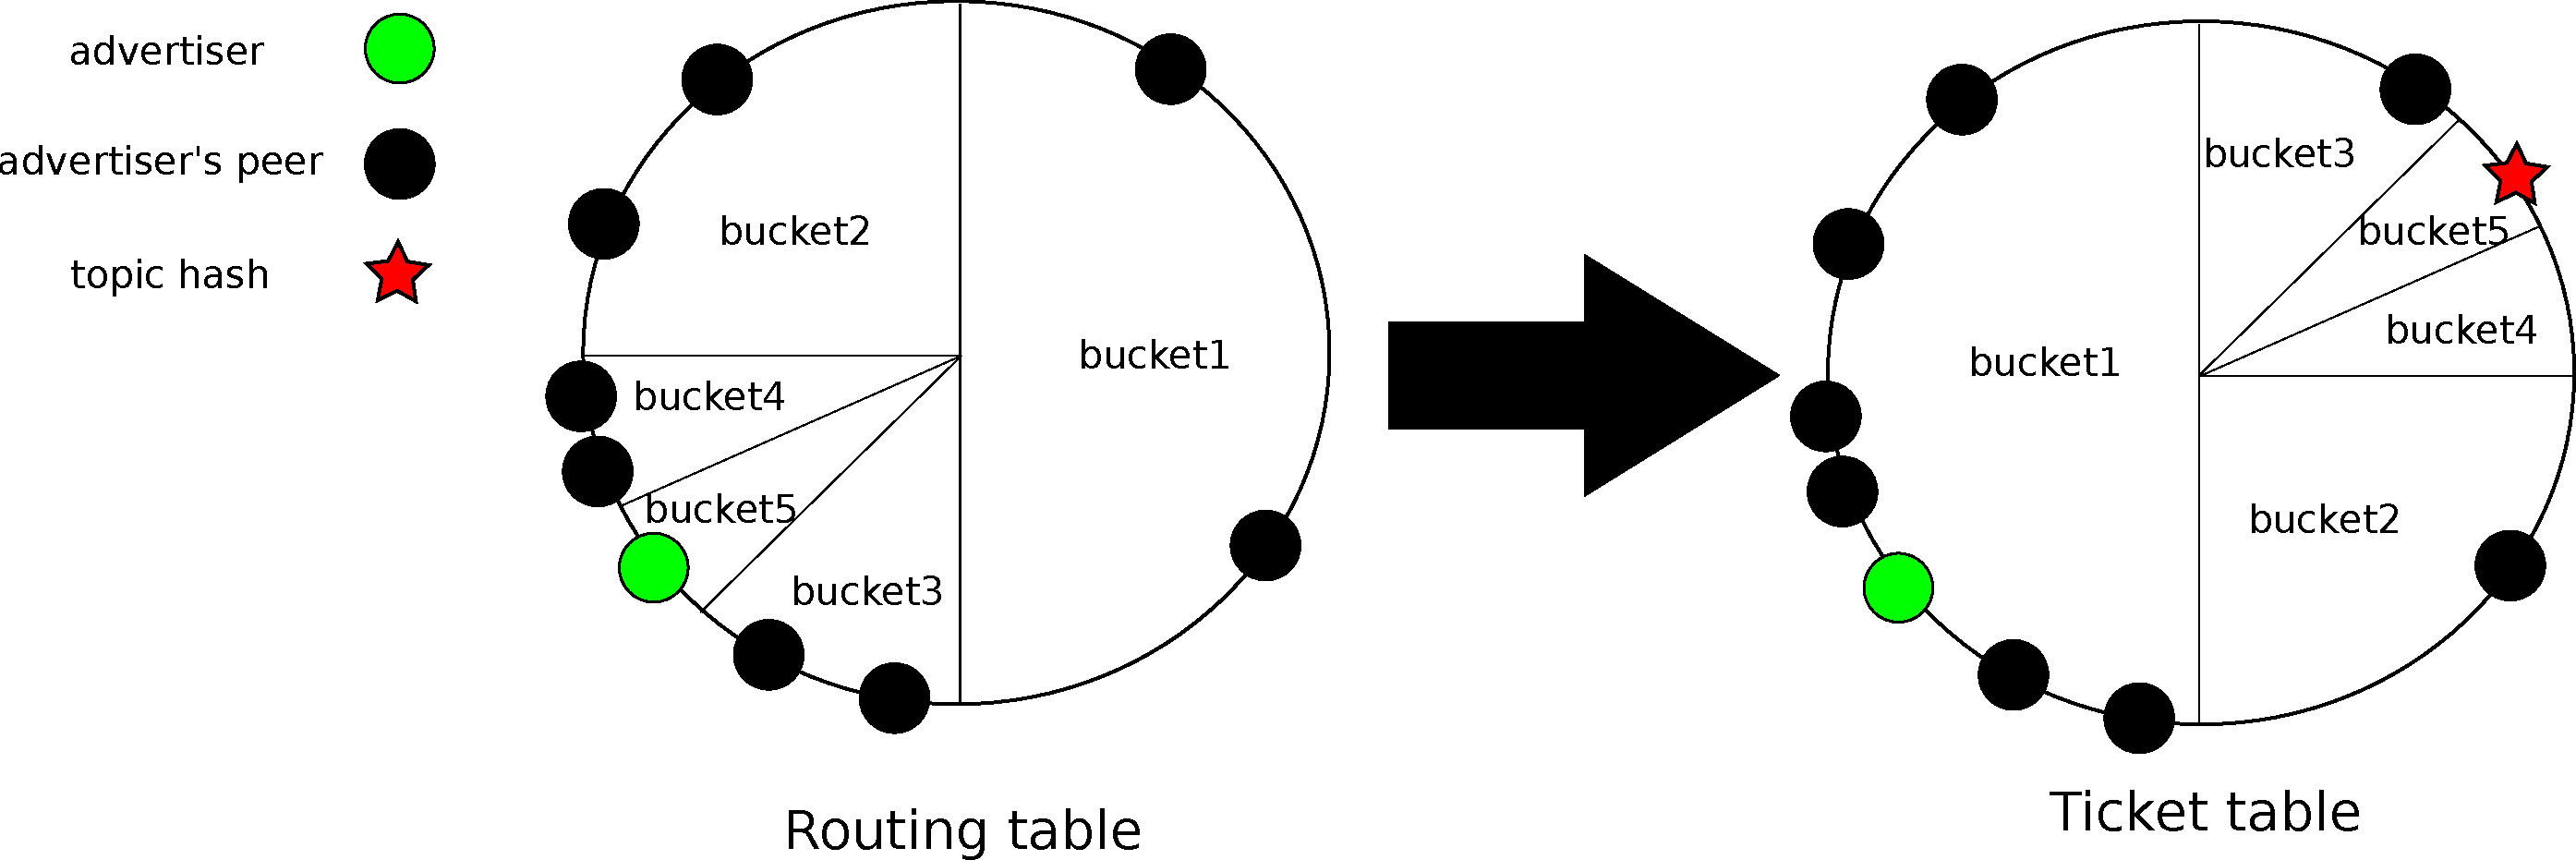
\includegraphics[width=0.45\textwidth]{img/ticket_table}
    \caption{Creation of ticket table from the routing table.}
    \label{fig:ticket_table}
 \end{figure}
 
 \para{How to ensure fairness with limited resources of the registrars in an open system with malicious nodes?} We assume the registrars will store ads in a fixed size \textbf{topic table}. The ad distribution procedure from above attempts to spread the load equally across nodes in the network. However, malicious nodes may decide to ignore the protocol trying to overload one or multiple registrars with their traffic. Furthermore, honest advertisers registering for large number of topics may exhaust limited resources of the registrars. 
 
 \sysname solves this problems by using a lightweight \textit{waiting-time-based admission mechanism}. When an advertisers sends an ad placement request to a registrar, the registrar will calculate an amount of time the advertisers needs to wait before being admitted (\ie the waiting time). The registrar also issues a \textbf{ticket} to the advertiser. The ticket specifies the time of the initial request, the calculated waiting time and is digitally signed by the registrar. The advertiser includes the ticket in its following registration requests and will be admitted only if the waiting is lower than the time the advertiser already waited for (as indicated by the initial request time). 
 
 The waiting time is calculated based on the diversity of the request (\ie how different is the request from ads already in the topic table?) and space left in the topic table. The more different the request is (in terms of the IP/ID of the registrar and the topic) from the current content of the topic table, the lower the calculated waiting time. At the same time, the calculated waiting time increases as the topic table fill in. The diversity score simplifies the admission for unpopular topic, as receive lower waiting times and are more likely to be admitted (\textbf{+G1, +G2}). Furthermore, high diversity of the topic table makes \sysname resistant to network dynamics (\textbf{+G7}). The proposed admission mechanism also prevents Sybil attacks performed by an attacker with a limited amount of resources (\textbf{+G8}). For instance, consecutive registration attempts from a single IP address will receive increasing waiting time eventually blocking further registration attempts made by the attacker. Including the current topic table size in the waiting time improves the load distribution. Registrars located close to the hashes popular topics will quickly will their topic table and return higher waiting times to the advertiser limiting the incoming traffic (\textbf{+G3}). 

%!TEX root = ../main.tex
%=========================================================

\section{Ads placement}
\label{sec:placement}
In the following, we provide a description of distributing advertisement in the network and discuss the process of search and establishing sub-protocol connections. 


\subsection{Data Structures}
We start by describing data structures necessary for topic-specific registrations and lookups. 

\para{Registration Table}
In order to execute the ad distribution process described below,  each advertiser maintains a per-topic \emph{registration table} for each advertised topic. The table keeps track of the ongoing registration attempts with different registrars.  The registration table is similar to the routing table used in Kademlia protocol (as described in \Cref{sec:background}). It stores advertiser's peers divided into k-buckets. However, instead of placing nodes in buckets based on the distance from the advertiser, it uses the distance from the topic ID. I.e. the registration table stores $k$ potential registrars for every distance range (bucket) from the topic ID (\Cref{fig:ticket_table}). When created, the table is initialized with peers from the routing table. 

\dk{Imo, it is not clear if there is a single topic table each node maintains, or if each node has one topic table for each Topic ID. Especially because the previous Section said there is a \emph{second} table for topics.}

\begin{figure}
    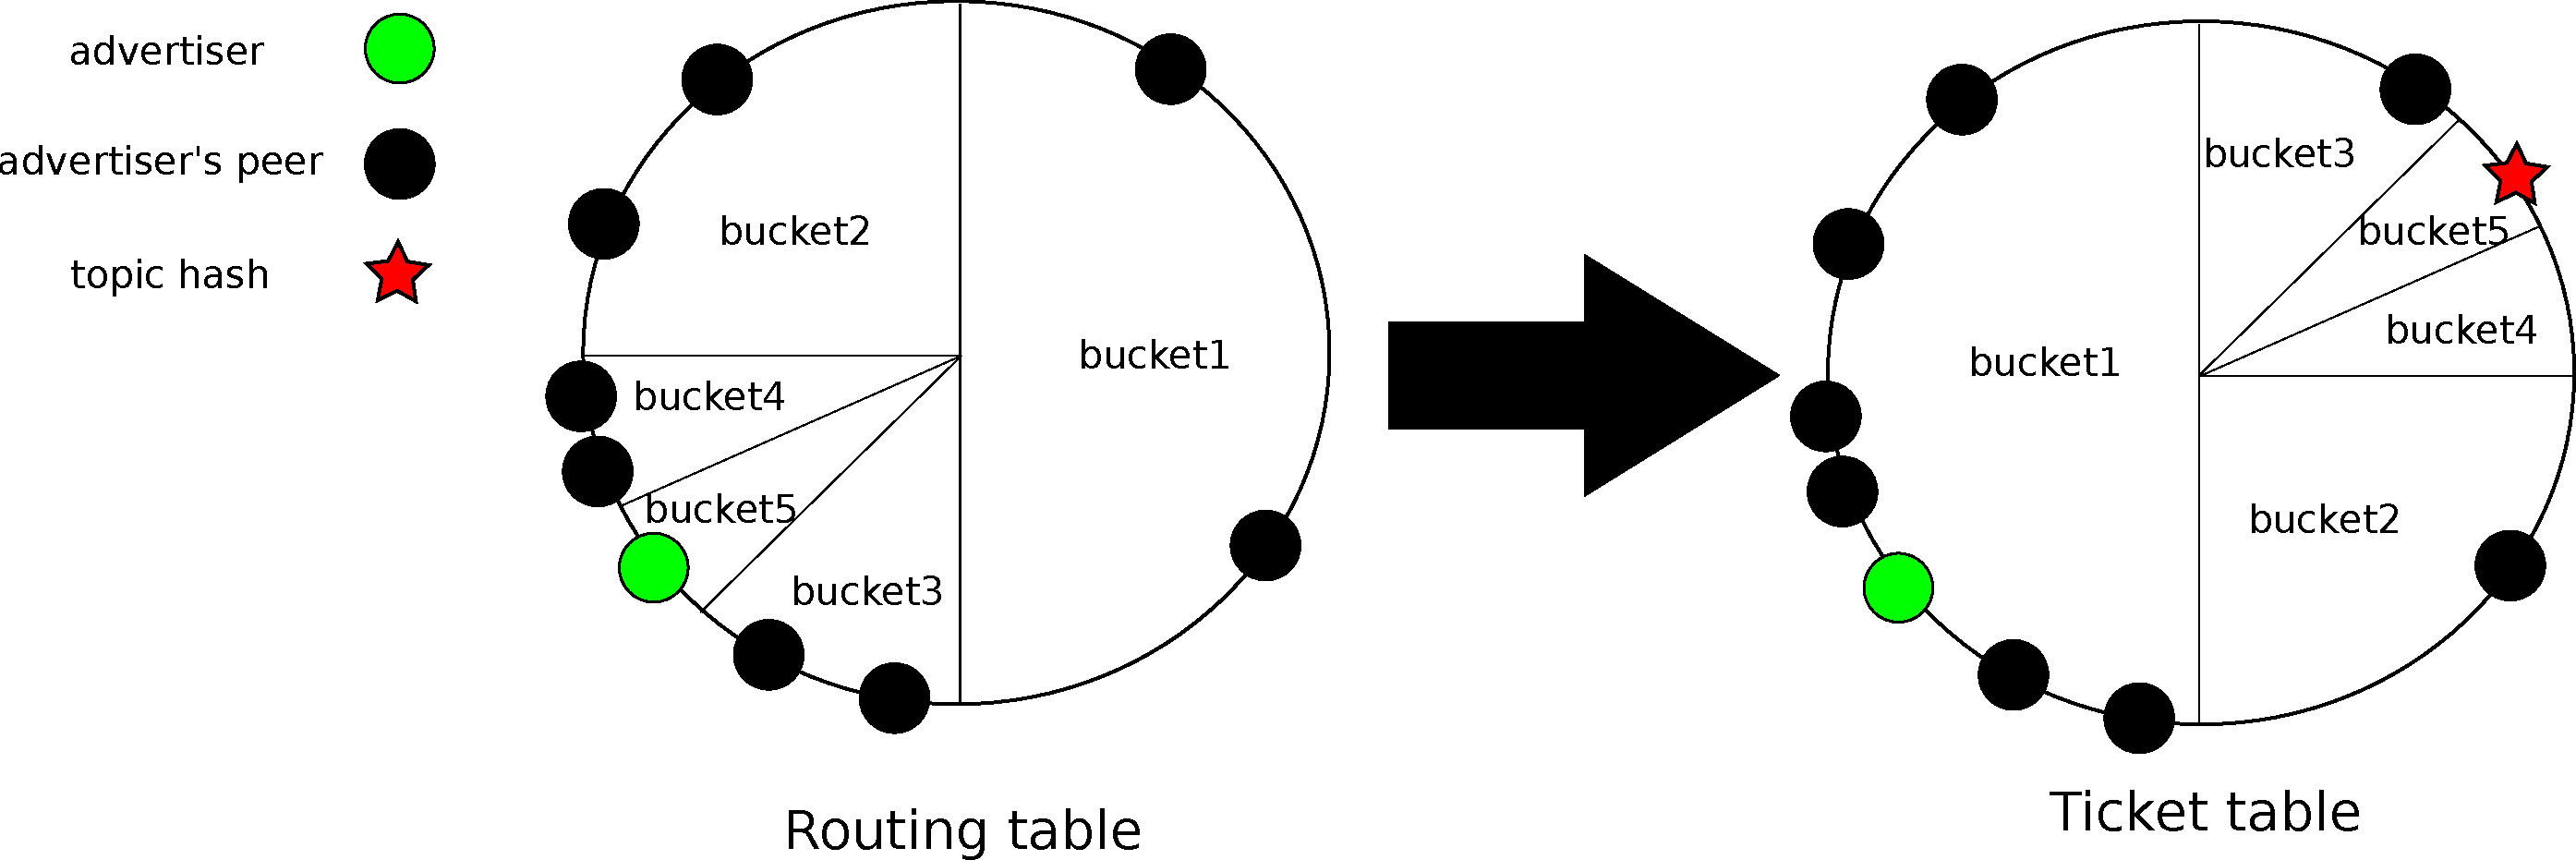
\includegraphics[width=0.45\textwidth]{img/ticket_table}
    \caption{Creation of ticket table from the routing table.}
    \label{fig:ticket_table}
 \end{figure}

\para{Search Table}
The ad lookup process is supported by a \emph{search table}. 
Searchers maintain a separate table per topic they are currently looking for. 
\ie for each topic the client wants to start discovering nodes, a new \emph{search table} is created. 
Similar to the \emph{registration table}, the \emph{search table} also stores k-buckets of registrar nodes by distance to the topic hash and buckets are initially filled from the local routing table organised by the distance from the topic hash.

%and a new 'search table' is created for each topic. 
%The bucket size \texttt{k}  of the search table should be relatively large in order to make the search efficient. 
%By default we use\texttt{k=16},  similarly to the local routing table (Kademlia DHT).
%Tickets are not required for search and nodes can not be added multiple times in the same k-bucket.

\subsection{Distributing ads across registrars}\label{sec:registration_multi}
When an advertiser wants to associate themselves with a topic, they start by creating a topic-specific \emph{registration table} (as described above). 
Every peer present in the registration table is a potential registrar. 
The objective of the ad placement process is to continuously maintain $K$ active (\ie unexpired) registrations in every bucket. 
Buckets located close to the topic hash cover less hash space than buckets located further away and, in turn, contain less potential registrars. 
Placing a fixed amount of ads per bucket, make registrars close to a topic hash more likely to receive registrations for that specific topic. 
Increasing $K$, makes the advertiser easier to find at the cost of increased communication overhead. 

The advertiser starts by the first bucket (the furthest away from the topic hash) in the \emph{registration table}, selects $K$ random peers and attempts to perform a registration. 
\dk{Why not all bucktes in parallel?}
We describe details on the registration procedure in \Cref{sec:registration}. 
A successful registration places an ad on an advertiser for a fixed amount of time $t_\textit{lifetime}$.
If a registration is unsuccessful (the selected registrar is down or refuses to store the ad), the advertiser selects another random peer from the same bucket and retries the registration process. 
The advertisers always maintains $K$ attempts and/or successful registrations per bucket unless less than $K$ peers are present in a specific bucket. 
The advertiser repeats the process for every bucket in the registration table. 
\michal{An algorithm here?}

As mentioned above, the \emph{routing table} is initialized with the peers already present in the routing table. It is thus possible that an advertiser will not know any nodes in buckets located close to the topic hash\footnote{This usually happens when the advertiser's ID is distant from the topic hash.}. 
To fill the empty buckets, the advertiser asks potential registrars to return $N$ closest peers to the topic hash they know of. 
The procedure is similar to the regular DHT \emph{FIND\_NODE} operation described in \Cref{sec:background}. 
The registrars respond with a list peers regardless of the success of the registration operation. 
The advertiser uses the returned information to populate its \emph{registration table}. 
As the advertiser progresses through the buckets, it queries potential registrars located closer to the topic hash and thus having a more detailed view of this part of the network. 
Similarly to the DHT routing, the registration procedure is guaranteed to find the closest node to the topic hash in the network. 
\ramin{Why not just use FIND\_NODE?}
\michal{It's basically FIND\_NODE but based on a different table (registration table, rather than the routing table) and performing the registration on top of traversing the DHT. IMO it's easier to have a seperate name here.}

%In addition to that, every time a node sends a ticket or registration request, the registrar replies with the closest nodes to 'the topic hash' that it knows. 
%This helps filling up k-buckets without sending additional lookups. 
%Also, when performing topic search (sending lookups for specific topics),  closest known nodes to 'the topic hash' are attached by the registrar node in the response.




\subsection{Lookup operation}\label{sec:lookup}
To find ads, \sysname uses a process similar to the registration procedure. 
The goal is to find $N_\textit{lookup}$ node advertised with a specific topic. 
The searcher starts by creating a topic-specific \emph{search table} initially populated with nodes from the \emph{routing table}. 
\michal{Should we have separate $K$ for registration and lookup? You might argue that if less ads are placed, more lookups are needed and vice-versa.}
\sergi{we actually use different values of $k$ for registration and search.  we could name it differently}
The searcher progressively moves through buckets (starting from the furthest away), randomly chooses $K$ registrars per buckets and sends them lookup requests. 
Each queried registrar responds with a list of $N_\textit{return}$ topic-specific advertisers the registrar know of. If the total number of topic-specific registrations is larger then $N_\textit{return}$, the registrar return a random subset. While both $N_\textit{return}$ and $N_\textit{lookup}$ are protocol parameters, the amount of ads returned by a single registrar must be lower than the total number of ads searchers are aiming to find $N_\textit{return} < N_\textit{lookup}$. It allows to diversify sources of ads received by the searcher. I.e., a single malicious registrar is not able to stop an honest searchers from contacting other nodes.
There is a tradeoff between overhead and security when choosing $N_\textit{return}$ and $N_\textit{lookup}$. 
By requiring a large amount of total ads to stop the search ($N_\textit{lookup}$) and low amount of ads returned by registrar $N_\textit{return}$ a higher diversity of data sources is achieved by the cost of contacting a large number of registrars. On the other hand, similar values of both $N_\textit{lookup}$ and $N_\textit{return}$ reduce the overhead but increase the danger of a searcher receiving ads uniquely from malicious nodes. Finally, low values of $N_\textit{lookup}$ stop the search operation early,  before reaching registrars close to the topic hash, contributing to more equal load spread. We investigate the impact of both parameters in \Cref{sec:eval}.
\ramin{In practice, is $N_\textit{lookup}$ a parameter that can be controlled? It sounds like something application-specific, e.g. for some applications, it might be enough for a searcher to just find one node to be able to use the application as intended. Search for 10 and choose one randomly from them?}
\michal{That's a good point. Not sure if we should allow the application to control both $N_\textit{lookup}$ and $N_\textit{return}$. Or maybe fix a ration between both and automatically set $N_\textit{return}$ once $N_\textit{lookup}$ is chosen by the application.}

Once ads are discovered,  the searcher can initiate topic-specific connections based on rules specified by the application. 
Applications do not only receive a list of potential nodes to connect but also the registrar node source of the search response.
In order to avoid eclipse attacks it is recommended not to start connections with nodes coming from the same registrar. 
Therefore connections are initiated always trying to keep the maximum diversity of the  registrars nodes used.
Once all nodes received have been used to try new connections,  a new search process is initiated. 

%\subsubsection{Updating connections}
%\michal{Didn't touch this subsection. Should it be here?}
%\sergi{i integrated some part in the last paragrah and the resti is already in the background section}
%Using the search results, a searcher updates its subprotocol-specific connections. 
%For instance,  each Ethereum client keeps connections towards 50 other nodes,  2/3 of those are for inbound connections (\ie 34 connections) where the client has no control over them, and the rest (about 16 connections) are four the outbound connections initiated towards the discovered nodes using the discovery protocol. 
%When a lookup is done,  the nodes discovered are stored in a buffer. 
%For each node of the buffer a connection is initiated. 
%The connection can be successful when the node targeted is alive and has empty slots in the inbound connections,  otherwise the connection is unsuccessful and a new node is selected.
%The nodes from the buffer are consumed as connections are attempted to the nodes.
%The buffer not only stores the nodes information but also the registrar node that replied with it.
%In order to avoid eclipse attacks it is recommended not to start connections with nodes coming from the same registrar. 
%Therefore connections are initiated always trying to keep the maximum diversity of the  registrars nodes used.

%\onur{need to explain this process since security depends on that.}

%All the modifiers from the first part of the equation increase with increasing number of the same items that are already in the table, i.e., reduction in diversity. Thus it's getting increasingly difficult to register ads for the same IP/ID/topic. For instance, ads for less popular topic will receive lower waiting times than popular ones. Note that the table does not prevent anyone from registering, but rather makes it slower for already popular items. Such a mechanism promotes diversity in the table and protects against Sybil attacks so that an attacker who is in control of a limited pool of IP addresses won't be able to dominate the table with many ads. The low exponent for the topics is motivated by the topics in the network that are likely to follow a skewed (e.g., a zipf-like) distribution. In contrast, honest nodes' IPs/IDs should follow a uniform distribution.

%The latter part of the formula is determined based on a multiple of ad-lifetime and the current utilisation (i.e., occupancy divided by capacity) of the table. When the utilisation becomes closer to 1.0, the base time becomes very large due to a very small denominator. Before the waiting time becomes infinite (when utilisation becomes 1), the waiting time becomes extremely high, in which case the advertisers give up as explained in the ad distribution process.

%The advertiser attempts to place an ad on each registrar and keeps the latest ticket issued by that registrar. It also keeps references to all pending tickets in a priority queue keyed by the expiry time of the ticket so it can efficiently access the next ticket for which a placement attempt is due.
%Since the table is limited to K values per bucket,  this means there are K on-going registrations per distance to the topic hash id. 
%The number of buckets used in the ticket table is a configurable parameter, but it is recommended to use small number of buckets,  instead of using a bucket per bit of the address space,  to avoid overloading registrars with IDs close to the topic hash. 
%Any node with a distance below the maximum distance minus the number of buckets will be stored in the same bucket.
%In our evaluation we used a ticket table with 10 buckets. 



%This objective is achieved by the advertisers setting a timer with a duration of ad-lifetime immediately upon the receipt of a REGCONFIRMATION from a node in a bucket b, and once the timer expires (after ad-lifetime passes) the advertiser starts a fresh registration with a node that is also located in bucket b. 
%The ticket table is used to store the tickets obtained for each on-going registrations and to keep track of the expiration times of active registrations.

%\subsubsection{Bucket refresh}

%The Ticket table needs to be initialised and refreshed to fill up all the per-distance k-buckets. 
%Ideally,  all k-buckets should be constantly full,  meaning that the advertisers place registrations at registrars in all distances to the topic hash. 
%An option to fill up all k-buckets would be to send periodic lookups for the specific distance to the topic hash, but since there are some distances that tend to be empty in the id space,  sending periodic lookups for the topic hash may create an additional overhead that can be too expensive and create too much traffic in the network. To avoid that, initially, the 'ticket table' k-buckets are filled performing local Ethereum routing table lookups to all distances to the 'topic hash' of the advertised topic.


%\michal{The below seems like an implementation detail.}
%There is  also a refresh bucket process,  similar to the Kademlia DHT table,  where periodically a random bucket is checked to see if it is empty.
%The \texttt{refresh time} is a configurable parameter. 
%We set a \texttt{refresh time=10 seconds} as a reference for our performance evaluation.
%During the refresh process,  in case the bucket checked is empty, 
%a local lookup to the Kademlia DHT table is performed. 
%In case no nodes have been found for the bucket distance,  a Kademlia lookup is performed towards the topic hash~\footnote{The lookup is performed by sending a FINDNODE message,  as described inhttps://github.com/ethereum/devp2p/blob/master/discv4.md.}
%Also, all nodes in the checked bucket are pinged to check they are still alive. 
%In case they are not, tickets for those dead nodes are removed from the ticket table and registrations to new nodes are initiated.




%We implemented and evaluated a lookup strategy that choose which nodes from which buckets ask first trying to diversify the nodes discovered as much as possible and trying not to overload nodes close the topic hash.
%A random node is picked from a bucket following a round-robin approach. 
%It starts picking a random node from the highest distance bucket and follows to the next distance in the bucket list.
%In order to find new results,  bucket entries are replaced when the node fails to answer or when it answers with an empty list of ads. 

%There is also a refresh process,  equivalent to the \emph{ticket table} refresh process, where random buckets are selected and all nodes in the buckets are checked for liveness.
%In case the bucket is empty a Kademlia lookup is performed towards the topic hash.


\section{Registration Protocol}\label{sec:registration_single}

\subsection{Data Structures}
\para{Topic Table}
Registrars store advertisers ads locally in a data structure called \emph{topic table}, 
indexed by advertisement topic. 
Each list of ads for a particular topic in the table  can be considered as a \emph{topic queue} because it functions like a FIFO queue.
Ads enter the queue once the registrar ticket is accepted,  and
the ad remain in the queue for a constant amount of time \texttt{target-ad-lifetime}. 
When \texttt{target-ad-lifetime} expires the ad is removed  from the queue.

\begin{figure}
    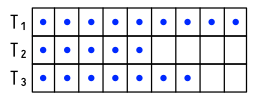
\includegraphics[width=0.35\textwidth]{img/topic-queue-diagram.png}
    \caption{Topic table structure.}
    \label{fig:topic_table}
 \end{figure}

The total size of the topic table is limited by \texttt{topic table capacity},  however there is no per-topic limits since existing number of topics in the network is unknown. 
Reasonable \texttt{topic table capacity} is 50,000 ads. 
Since ENRs are at most 300 bytes in size, these limits ensure that a full topic table consumes approximately 15MB of memory.
An advertiser can only place a single ad for a specific topic queue in the topic table at the same time; duplicate placements are rejected (although the same node may attempt placing ads for multiple topics at the same registrar).

The topic table is shared across multiple advertisers and stores topics with varying popularity (which is determined by how many nodes register the topic) among the participants of \sysname. 
It is important that the high popularity of a particular topic should not prevent peers from registering less popular topics. 
This is achieved using the waiting time function that will determine the time an advertiser will have to wait to place an ad after a ticket request,  and is detailed in Section~\ref{sec:waitingTime}.

\subsubsection{Registration Procedure}

In order to place an ad on a registrar's topic table,  the advertiser must present a valid 'ticket' to the registrar. 
%Tickets are immutable objects issued by the registrars. 
Tickets are immutable objects storing arbitrary information determined by the issuing registrar node.  While details of encoding and ticket validation are up to the implementation, tickets must contain enough information to verify that:
\begin{itemize}
    \item The advertiser attempting to use the ticket is the one which originally requested it.
    \item A ticket is valid for a single topic only.
    \item A ticket can only be used within the 'registration window' (explained below).
    \item A ticket can not be used more than once.
%     \michal{Can we enforce it? I can use the same ticket twice within the validity period, right?\onur{It seems possible for an advertiser to essentially duplicate an existing ticket by using it twice during the validity period. The duplicate ticket gets a new waiting time, accumulates a high cum. waiting time so that the advertiser can re-register its ad with significant advantage over other contenders. I think an easy fix is for registrars to drop/ignore tickets for which there is an active registration. }}
\end{itemize}

An advertiser willing to register an ad at a registrar must first obtain a ticket from that registrar by sending a 'ticket request' (TICKETREQUEST) message to the registrar. In response to the ticket request, the registrar issues an initial ticket containing a 'waiting time' and sends the ticket to the advertiser in a 'ticket response' message. The advertiser can come back to the registrar (to register an ad) after the waiting time has elapsed and present the ticket in a 'topic registration request' (i.e., REGTOPIC) message.

\michal{Change the markdown notation of variables (CAPACITY) to scientific (n)}
Any REGTOPIC messages that are not sent during the registration window determined by the waiting time (indicated in the ticket),   (as seen in Figure \ref{fig:ticket_validity}) are ignored by the registrars.  
If the advertiser comes back during the established registration window,  the advertiser can either place the ad (and notify the advertiser of a successful registration) or issue another ticket with a new waiting time in another ticket response message. 
An advertiser may be given one or more tickets in a sequence before a successful registration,  and this means that overall the advertiser waits for a 'cumulative waiting time' period that is the sum of multiple waiting times issued in each ticket in the sequence before finally registering an ad. 
Assignment of 'waiting times' is the only way the registrars can control the registrations in order to both:

\begin{itemize}
    \item Throttle ad placement rate to prevent overflowing of topic table: when the topic table is full, the advertisers must wait for already placed ads to expire first before they are allowed to register new ads.
    \item Prioritise registrations to achieve a diverse set of ads in the topic table. For example, registrations for less popular topics or registrations from advertisers that increase IP diversity (in the set of advertiser IP addresses that currently have an ad in the table) can be prioritised over others. This is useful to reduce the impact of Sybil attacks on the service discovery system.
\end{itemize}

Waiting times will be calculated according to a 'Waiting time function' detailed in Section~\ref{sec:waitingTime}.  Enforcing this time limit prevents misuse of the topic table because any topic must be important enough to outweigh the cost of waiting for ad placement. Imagine a group phone call: announcing the participants of the call using topic advertisement isn't a good use of the system because the topic exists only for a short time and will have very few participants. The waiting time prevents using the topic table for this purpose because the call might already be over before everyone could get registered. Also, it prevents attackers from overflowing topic table by regulating registrations in case of spamming attacks.

Tickets cannot be used beyond their lifetime. If an advertiser does not come back after the waiting time, all cumulative waiting time is lost and the advertiser must start over (\Cref{fig:ticket_validity}). When the ticket is issued, the node keeping it must wait until the registration window opens. The length of the registration window is implementation dependent, but by default 10 seconds is used. The ticket becomes invalid after the registration window has passed. This mechanism prevents malicious advertisers from obtaining a ticket, then just wait for a long time until a large cumulative waiting time is accumulated, and finally launch a coordinated attack to take over the topic table with their ads.

In addition to the waiting time,  the sequence of tickets issued by a registrar for a specific advertiser also records the original issue-time of the first ticket which can be used to compute the cumulative waiting time so far; that is, the time elapsed since the advertiser requested its first ticket to place its ad. The inclusion of issue-time allows the registrars to prioritise advertisers that have been waiting the most as we explain later. Because the tickets are immutable (i.e., tampering with the ticket is detectable by the registrars that originally issued the ticket), when a registrar issues a new ticket (in case a registration is not immediately successful) to an advertiser, the registrar simply copies the issue-time from the last issued ticket and use that as the issue-time of the new ticket. This means that the registrars are not required to maintain any state for each on-going ticket request given that they can simply verify the authenticity of the ticket in the incoming registration requests. 
%The registrars ensure the authenticity of the tickets they issue to the advertisers through symmetric encryption we explain below.

    
\begin{figure}
    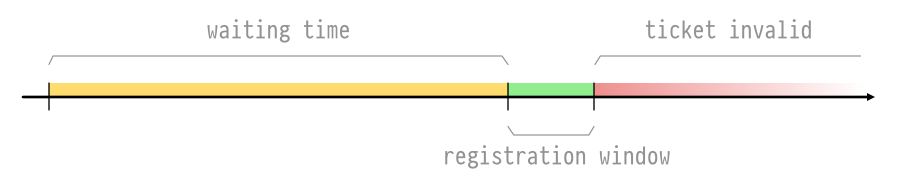
\includegraphics[width=0.5\textwidth]{img/ticket-validity}
    \caption{Ticket validity period.}
    \label{fig:ticket_validity}
\end{figure}


\michal{We're mixing here single-registrar registration process. It should be covered in the first section.}
In our approach,  advertisers start a limited number of parallel registrations in each ticket table bucket distance.
 More specifically, an advertiser follows the below steps to distribute its ads for a specific topic:
\begin{enumerate}
     %\item The advertiser (\hl{randomly?}) selects a set of K registrar nodes from each bucket distance of the ticket table structure, where the number of bucket distances (B) is a configurable parameter of the ticket table.
    \item The advertiser selects a K random of node.,  by querying the local Ethereum routing table,  for each bucket distance.
    \item A TICKETREQUEST message is initially sent to each of the selected registrar nodes in the previous step.
    \item Registrar node replies with a TICKETRESPONSE.  This message includes the TICKET which contains a waiting time and a ticket issue time.  The TICKET is stored in the table.
    \item The advertiser replies after the waiting time expires with a REGTOPIC request containing the previously received TICKET attached to it.
    \item After the TICKET reception the waiting time is calculated again at the registrar.  A registration is successful when the waiting time calculated at the registrar is smaller than the cumulative waiting time,  which means that the advertiser has waited long enough.
    \item The registrar sends a REGCONFIRMATION response to the advertiser of the successful registration. In general, the topic table occupancy is guaranteed to always remain below the topic table capacity by the waiting time calculated: the waiting time function returns increasingly large values as the topic table space runs out; the waiting time becomes infinite in case there is no space.
    \item In case the new calculated waiting time is not smaller than the cumulative waiting time, the registration is not successful and the registrar replies with a REGRESPONSE message containing a new TICKET (containing a new waiting time).
    \item A registrar gives up and stops the registration process with a registrar (say R) upon either T unsuccessful registration attempts (i.e., after being issued T tickets in REGRESPONSE messages from the registrar without a REGCONFIRMATION) or receipt of a ticket with a waiting time larger than LARGEWAIT value.  In that case,  the advertiser removes it from the ticket table and selects a new node located in the same bucket as R until filling K and the process is restarted (step 1).
    \item Similarly,  after the expiration of a previously placed ad (i.e., after the passage of ad-lifetime upon receiving a REGCONFIRMATION message) the node is removed from the ticket table and the process is restarted with a new node picked from the local table (step 1).
\end{enumerate}

%\section{Goals recap}

\subsection{G1 - all the registrants  should be able to place their advertisements in the network.}

\subsubsection{Mechanism developed:} 

Proposed registering mechanism + waiting time function that 

\subsubsection{Evaluation: }


- Registrations per topic graph (compared with nodes registering per topic).  

- Registrations per node

- topic table graphs (python)

\subsection{G2 -  all the registrants within each topic should have a similar probability of being discovered}

\subsubsection{Mechanism developed:} 

In the proposed registration mechanisms all nodes within a topic have the same probability of placing advertisements in other nodes,  although can be biased depending on the ip limitation (e.g. nodes from same /24 subnet) and bucket structure.

In the same way,  nodes are equally discovered. 
May be that nodes that place registrations in closest distance buckets are more discovered, although all have same chances to get in. 
Also search start from furthest buckets,  so maybe no really affecting. 
 (check this)
 ( existing graph may be not accurate enough)

\subsubsection{Evaluation: }

Registrant distribution graph. \sergi{I would redo this graph to make it more accurate}/

\subsection{G3 - the load should be equally distributed across all the nodes}

\subsubsection{Mechanism developed:} 

The bucket structure of the DHT could lead to more traffic and therefore discoveries for certain nodes in the network.  However, waiting time function makes it more difficult to register on those nodes and therefore limiting traffic received.
However, since nodes on closest buckets are discovered by everyone when joining the network,  this provides some deviation on the  distributed load.  

\subsubsection{Evaluation: }

Load graph. 
We should evaluate also based on the lifetime of nodes
and with different turbulence rates to see how it 
affects closest bucket nodes.

\subsection{G4 - the registration operation should be efficient in terms of time}

\subsubsection{Mechanism developed:} 

Time to registration if strictly depends on the popularity of the topic. 
Registrations with no previous registrations for a specific nodes have priority and therefore are very fast.

\subsubsection{Evaluation: }

Time to registration graph

\subsection{G5 - the registration operation should be efficient in terms of overhead}

\subsubsection{Mechanism developed:} 

The number of messages required to place registrations is bounded

\subsubsection{Evaluation: }

Overhead graph

\subsection{G6 - the lookup operation should be efficient in terms }

\subsubsection{Mechanism developed:} 

Hopcount and time necessary to discover nodes is bounded thanks to buckets structure for the discovery.

\subsubsection{Evaluation: }

Lookup hopcount graph
Lookup time ???? 

\subsection{G7 - all topics should be able to be discovered}

\subsubsection{Mechanism developed:} 

Registration and discovery mechanism ensure any node can place registrations and be discovered regardless of the popularity of the topic. 
Even for a single node topic, it should be able to be discovered in the network 

\subsubsection{Evaluation: }

Lookup hopcount and registrant discovery 
for different popularity topics

\subsection{G8 - the protocol should be resistant to network dynamic (nodes joining leaving)}

\subsubsection{Mechanism developed:} 

Registrations are dynamic and expiring after certain time. 
New nodes joining the network are able to place registrations in the network and, as old registrations expire,  new nodes are able to place theirs advertisements in equal conditions.

\subsubsection{Evaluation: }

Nodes registration graphs comparing with turbulence.

\subsection{G9 - the protocol should be resistant to sybil attacks launched by malicious nodes}

\subsubsection{Mechanism developed:} 

Waiting time function is designed to limit the number of sybils can place registrations.

\subsubsection{Evaluation: }

All attacks evaluation

%\begin{itemize}
%    \item 
%    
%    \item G2 - all the registrants within each topic should have a similar probability of being discovered by their peers.
%    \item G3 - the load (in terms of sent and received messages) should be equally distributed across all the nodes regardless of their ID and location in the network
%    \item G4 - the registration operation should be efficient in terms of time (fast) for all the registrants
%    \item G5 - the registration operation should be efficient in terms of overhead (low amount of sent/received messages) for all the registrants
%    \item G6 - the lookup operation should be efficient in terms of time (fast) and messages sent (hop count) for all the query nodes
%    \item G7 - the number of registrations should be sufficient for an efficient discovery of nodes despite the popularity of the topic
%    \item G8 - the protocol should be resistant to network dynamic (nodes joining leaving)
%    \item G9 - the protocol should be resistant to sybil attacks launched by malicious nodes
%\end{itemize}
\section{Waiting Time}
\label{sec:waitingTime}
The waiting time function is used to calculate the total time advertisers have to wait before being admitted to the topic table. 
The function directly shapes the structure of the topic table,  determines its diversity and performs flow control. 
It also protects against attacks, where a malicious actor tries to dominate the topic table and exhaust resources of the registrar. 

Each request is given a waiting time based on the IP address of the registrar, the ID of the registrar, the topic of the request and the current occupancy of the topic table. 
The waiting time function is divided into two parts: \emph{occupancy score} and  \emph{similarity score}. The final result is a product of both scores: $w =  \textit{occupancy score} \times \textit{similarity score} $. 

The \emph{occupancy score} is based uniquely on the number of the ads already in the table.
Its role is to progressively increase the waiting time as the topic table fills up and to limit the memory used by a registrar.
The \emph{occupancy score} is defined by equation~\ref{eq:occupancy}:

\begin{equation}
\label{eq:occupancy}
    \textit{occupancy score} = \frac{ba}{(1-\frac{d}{n})^{P_{occupancy}}}
\end{equation}
where $a$ is the \emph{ad lifetime} (the amount of time each ad spend in the topic table), $d$ is the number of ads in the table, $n$ is the capacity of the table. $b$ and $P_{occupacy}$ are protocol configurable parameters. 
When the number of ads in the table is low ($d \ll n$ ), the \emph{occupancy score} goes to $ba$. 
As the topic table fills up, the score will be amplified by the divisor of the equation. 
The higher values of $P_{occupancy}$, the faster the increase. 
With the current occupancy $d$ close to the capacity of the table $n$, the \emph{occupancy score} goes to infinity thus limiting the number of admitted requests. 

The role of the \emph{similarity score} is to determine how similar is the incoming request to the ads already in the topic table in terms of the IP address, the ID and the topic. 
Requests significantly different from the current content of the table receive lower similarity score resulting in lower overall waiting time. 
Such an approach promotes fairness across topics (it is easier for less popular topics to get into the table) and protects against attempts to fill the topic table by a small number of advertisers (as identified by their IP addresses and IDs). The similarity score is defined as a sum of similarity score for IP, ID and the topic of the request: $\textit{similarity score} = \textit{similarity score(IP)} + \textit{similarity score(ID)} + \textit{similarity score(topic)}$. 

The similarity score for ID and topics is the same given by the equation~\ref{eq:similarity}:
\begin{equation}
\label{eq:similarity}
    \textit{similarity score(topic)}= (\frac{d(topic)}{d})^{P_{topic}} 
\end{equation}
where $d(topic)$ is the number of ads for the specified topic already in the table, $d$ is the total number of ads in the table and $P_{topic}$ is a protocol parameter. 
The score goes to $1$ as the specified topic dominates the table $d(topic)  \approx  d$. 
Lower values of parameter $P_{topic}$ cause the similarity score to converge to $1$ faster. 

However,  for calculating the IP address diversity we use a different similarity score. 
A simple similarity score used for IDs and topics cannot be applied for IP addresses. 
An attacker may be able to generate a large number of different addresses sharing the same prefix (\eg using a single /24 IPv4 network) that, while similar, would receive low \emph{similarity scores}. 
Go Ethereum client~\footnote{https://github.com/ethereum/go-ethereum} limits the number of IP addresses coming from the same (\eg /24 IPv4 address) network. 
However,  it is impossible to reliably set those limits without knowledge about the network size or NAT configuration of honest nodes. 
Instead, we propose an approach that directly captures the similarity level across different IPs and translates it into a numerical score. 

We introduce a binary \emph{tree},  as shown on \Cref{fig:ip_tree},  that stores IP addresses used in the existing registrations in the topic table. 
Each node stores a counter,  while the edges represent consecutive $0$s or $1$s in a binary representation of IP addresses. 
For simplicity,  we present the \emph{tree} for IPv4 addresses but its adaptation for IPv6 is straightforward. 

\begin{figure}
    
\includegraphics[width=0.45\textwidth]{img/ip_tree}
    \caption{Inserting an IP address into the IP \emph{tree} structure.}
    \label{fig:ip_tree}
\end{figure}

Apart from its root,  the \emph{tree} consists of 32 levels (33 levels in total) representing bits in the binary representation of IPv4 IP addresses. 
The root level is depicted as level $0$, the level of its successor as level $1$ and so on. 
The counter of every \emph{tree} node is initially set to $0$. When adding an IP to the \emph{tree},  the address is first converted to its binary representation and follows a path in the \emph{tree} corresponding to consecutive bits. 
Counters of all the visited nodes are increased by $1$. 
As a result, the root counter stores the number of all the IP addresses in the topic table, its $0$ successor stores the number of the IP addresses starting with $0$, its $1$ successor stores the number of the IP addresses starting with $1$ and so on. 
Removing an IP from the \emph{tree} follows the analogical procedure but decreases all the counters on the path. 

After each addition of an address to the \emph{tree} a score is generated.
The score is a sum of counter values of visited nodes raised to the power of the node level. 
\michal{Probably need an equation here but not sure how to write it down. Maybe @Ramin could help?} 
The counter values are taken \emph{before} the increment caused by adding the address\footnote{The first added address will thus always have a score of $0$}. 
Finally,  the similarity score for an IP is defined by:
\begin{equation}
    \textit{similarity score(IP}) = (\frac{\textit{score(IP)}}{-(\textit{rootCounter})(1 - 2^{33})})^{P_\textit{IP}}
\end{equation}
The divisor of the equation represents the maximum possible score. 
That is, a score obtained if all the IP addresses in the \emph{tree} would be the same as the one being added. 
Similarly to ID and topic score,  the IP similarity score range from $0$ to $1$ and returns values closer to 1 for different addresses sharing the same prefix (the longer the shared prefix, the higher the score).

The final formula for the waiting time function can be represented with  the following formula,  adding all \emph{similarity scores} and multiplying by the \emph{occupancy score}:

\begin{equation}
\begin{split}
    \textit{w(IP, ID, topic)} = 
    (\frac{\textit{score(IP)}}{-(\textit{rootCounter})(1 - 2^{33})})^{P_\textit{IP}} + \\
    + (\frac{d(ID)}{d})^{P_{ID}} +
    (\frac{d(topic)}{d})^{P_{topic}})
    \frac{ba}{(1-\frac{d}{n})^{P_{occupancy}}}
\end{split}
\end{equation}

The formula can be simplified like in equation~\ref{eq:simp}, where ss determines the the \emph{similarity score} and os the \emph{occupancy score}.

\begin{equation}
\label{eq:simp}
    \textit{w(IP, ID, topic)} = 
    (\textit{ss(IP)} + 
    \textit{ss(ID)} + 
    \textit{ss(topic)})
    \textit{os()}
\end{equation}

\subsection{Lower Bound}
With the waiting time formula, every change in the registrations stored in  the topic table may increase or decrease waiting times of other requests. 
Therefore,  an advertiser receiving waiting time $w(t_1)$ at time $t_1$, may get a smaller waiting time $w(t_2)$ at time $t_2$ ($t_1 < t_2$) in case the situation of the topic table is very different (\eg when an ad for the same topic expires between $t_1$ and $t_2$). 
As a result,  advertisers willing to minimize their waiting time can be incentivized to keep checking the waiting time as frequently as possible hoping for a better one.
However, this can be a problem. 
Registration ticket requests should be kept to the minimum and an incentive for constantly spamming ticket requests to get a better waiting time can overload a network and can lead to some nodes getting better performance than the rest.
Thus we designed a mechanism to avoid that any node that is already in possession of a ticket with a determined waiting time,   can get a better waiting time (including the new waiting time and the time passed between the first ticket request and the subsequent) by issuing new ticket requests.
One solution to this problem is to take into account all the expiration times when calculating the waiting time. 
However, such a solution is computationally expensive (\eg $O(n)$) and unfeasable in practice.

\begin{figure}
    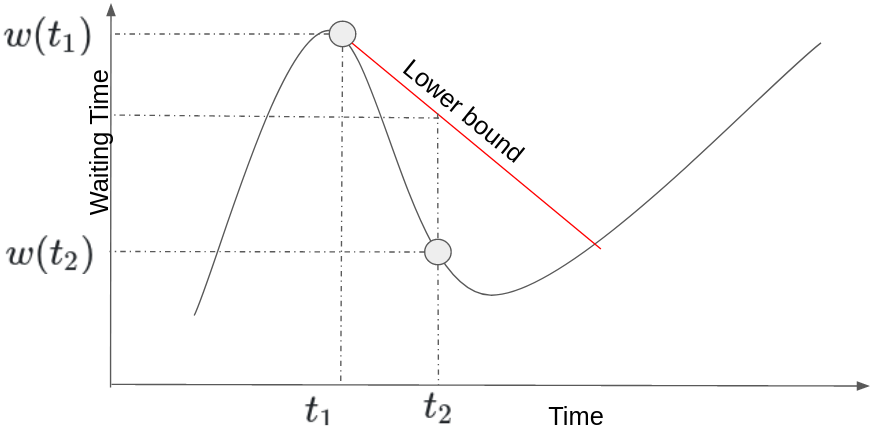
\includegraphics[width=0.45\textwidth]{img/lower_bound.png}
    \caption{Waiting time lower bound.}
    \label{fig:lower_bound}
\end{figure}

When asking for a new waiting time before the previously obtained one elapses, an advertisers loses its already accumulated waiting time . It means that asking for a new waiting at time $t_2$ can lower the overall waiting only if the new waiting time is $w(t_2)$ is smaller than $w(t_1)$ by more than $t2 - t1$: $w(t_1) - w(t_2) < t_2 - t_1$.
To make sure it is not the case,  our protocol enforces a lower bound on the waiting time. \Ie we make sure that a advertiser's waiting time received at $t_2$ is not smaller than the waiting time at $t_1$ ($t_1 < t_2$) by more than $t2 - t1$ (\Cref{fig:lower_bound}). 
However, holding such a bound for every request (\ie every combination of IP/ID/topic) would cause significant memory overhead ($O(|IPs|\times|IDs|\times|topics|)  \gg O(d)$) and would present an easy way for an attacker to create state at the registrar. 

To store the lower bound in a more efficient way, we rewrite the waiting formula as a sum of topic/IP/ID distinctive parts:

\begin{equation}
    \textit{w(IP, ID, topic)} = 
    \textit{ss(IP)}\textit{os()} + 
    \textit{ss(ID)}\textit{os()} + 
    \textit{ss(topic)}\textit{os()}
\end{equation}
Ensuring that the lower bound is enforced for each of the three components makes sure that the total waiting will respect the lower bound as well. At the same time, it only requires storing lower bound for every IP/ID/topic and not all their combinations. This approach reduces the memory overhead to $O(|IPs|+|IDs|+|topics|) = O(d)$.

For each of the components above IP, ID and topic present in the table, we keep a bound. When a specific IP enters the table for the first time, the bound(IP) is set to 0 and a timestamp timestamp(IP) is set to the current time. When a ticket request arrives from the same IP, we calculate the IP waiting time $w_{IP}$ and return the higher value among $w_{IP} = max(w_{IP}, bound(IP) - timestamp(IP))$. It makes sure that advertisers never receive a better time by frequently coming requesting new tickets. The bound and the bound are updated when a new ticket is issued and $w_{IP} > (bound(IP) - timestamp(IP))$. The same holds for IDs and topics.




%!TEX root = ../main.tex
%=========================================================

\section{Performance Evaluation}
\label{sec:eval}
%
%In  this  section,  we  provide  a  detailed  investigation  of  the performance of the proposed discovery scheme.
%We present the performance evalution in three different subsections. 
%In the first one we evaluate the performance of our novel waiting function by measuring the ticket table occupancy
%according with our design goals and parameters.
%The second one is a thorough performance evaluation under different scenarios, including Sybil attacks, of the whole network discovery solution using a peer-to-peer network simulator.
%In the third one we include an evaluation using the most used Ethereum client software, Geth~\cite{go-ethereum}, in a testbed scenario.

%\subsection{Ticket table occupancy evaluation}

%\sergi{Ticket table occupancy and waiting time evaluation TBC}

%\subsection{Network simulator evaluation}

%\sergi{TODO: modify figures with bigger fonts}
%\sergi{TODO: registrant distribution is not very readable. probably should be redesigned}
%\sergi{TODO: Lookup performance should be compared with something. Discv4? }

\subsection{Evaluation Setup}

For the  performance evaluation of the proposed discovery scheme. we extended the existing  large-scale peer-to-peer network simulator PeerSim~\cite{p2p09-peersim}.
We implemented the current Discv5 protocol by modyfing the available PeerSim Kademlia implementation with the differences of the Kademlia version used by the Ethereum network, and developing our solution on top of it. 
We make the code publicly available for the scientific community\footnote{https://github.com/datahop/p2p-service-discovery}.

\begin{table}[!hbt]
\centering
\scriptsize
\begin{tabular}{|c|c|}%|c|c|}
\hline
Parameter     & Value (\%) \\
\hline
\hline
%Network size & 2000 nodes \\%&  0.4321 & 0.8883\\
%\hline
Simulation time & 4 hours \\%& 0.7569 & 0.9959\\
\hline
Kademlia bucket size & 16 \\%& 0.6104 & 0.8515\\
\hline
Kademlia buckets & 17 \\%& 0.8225 & 0.9897\\
\hline
Ticket table bucket size & 5 \\%& 0.8225 & 0.9897\\
\hline
Ticket table buckets & 10 \\%& 0.8225 & 0.9897\\
\hline
Lookup table bucket size & 16 \\%& 0.8225 & 0.9897\\
\hline
Lookup table buckets & 17 \\%& 0.8225 & 0.9897\\
\hline
Registration lifetime & 15 minutes \\%& 0.8225 & 0.9897\\
\hline
Registration waiting time limit & 15 minutes \\%& 0.8225 & 0.9897\\
\hline
Number of topics & 5 \\%& 0.8225 & 0.9897\\
\hline
Number of topics & 5 \\%& 0.8225 & 0.9897\\
\hline
Zipf dist exp & 0.7 \\%& 0.8225 & 0.9897\\
\hline
Ticket table capacity & 500 \\
\hline
Turbulence event & Every 144 seconds per 1000 nodes. \\%& 0.8225 & 0.9897\\
\hline
Num of connections & 50 \\%& 0.8225 & 0.9897\\
\hline
\bottomrule
\end{tabular}
\vspace{2mm}
\caption{Evaluation scenario parameters}
\label{tab:param}
\vspace{-0.05in}
\end{table}

In Table~\ref{tab:param} we show the parameters used in the simulation. 
We performed 4 hours long simulations with different number of nodes from 500 to 10000.
In the simulations there are 5 different topics and all nodes participate in at least one topic (t1).\michal{We need simulations with more topics. 5 is just not enough.}
There is turbulence in the simulation,  \ie new nodes are added to the network and existing nodes are removed at a rate of one event every 144 seconds per each thousand nodes in the network.\michal{We 144? Do we have any churn data from Ethereum?}
Nodes are modelled similarly to an Ethereum client. 
When a node joins the network it starts advertising for the participating topics.
Each node has a pool of connections (separated by outgoing and incoming connections) for each topic in which they participate, and it perform lookups
for a specific topic to start connections with discovered nodes.
When an initial lookup is done,  the discovered nodes are stored in a buffer per topic.
Nodes start attempting connections with the discovered nodes from the buffer until all connections  are full.
In case the connection is possible (the targeted node has an available slot in the pool of connections and the node is still up), it is added 
to the local list of connections.
Nodes are removed from the discovered nodes buffer for each attempt of connection.
When a node goes down, a connection attempt is made with a new nodes from the buffer to occupy all available connection slots.
When the discovered nodes for a certain topic is empty, a new topic lookup is performed.
Nodes have a pool of 50 connections available, 16 for outgoing connections and 34 for incoming.

%\begin{table}[!hbt]
%\centering
%\scriptsize
%\begin{tabular}{|c|c|}%|c|c|}
%\hline
%Topic & 500 Nodes & 1000 Nodes & 5000 nodes & 10000 nodes \\
%\hline
%\hline
%T1 & 500 nodes & 1000 nodes & 5000 nodes & 10000 nodes \\%&  0.4321 & 0.8883\\
%\hline
%T2 & 1272 nodes \\%& 0.7569 & 0.9959\\
%\hline
%T3 & 803 nodes \\%& 0.6104 & 0.8515\\
%\hline
%T4 & 496 nodes \\%& 0.8225 & 0.9897\\
%\hline
%T5 & 218 nodes \\%& 0.8225 & 0.9897\\
%\hline
%\bottomrule
%\end{tabular}
%\vspace{2mm}
%\caption{Nodes per topic}
%\label{tab:nodes}
%\vspace{-0.05in}
%\end{table}


%\subsubsection{Results}

%\paragraph{\bf{Active registrations}:}

\subsection{Performance Results}
\michal{We should group the result so that they show achievement of specific goals that we described before}

%\paragraph{Ticket registrations:
In the following we detail the performance evaluation in four different subsections.  In the first we show the registration performance.  Secondly we show the traffic load and overhead of the designed mechanism.  Then we continue with the lookup and discovery performance and we finish with the security analysis.

\subsubsection{Registration  performance}

In Figure~\ref{fig:regs} we observe the average active registrations in the system per topic with different number of nodes in the simulation,  from 500 to 10000 nodes. 
We can observe nodes for all topics are able to place a substantial amount of registrations, even the less popular topics. 
As number of nodes increase in the network, we can observe the differences between registrations per topic are reduced. 
Actually, it can be observed the most popular topic (t1) is able to place less registrations than t2. 
This is caused by the fact that with more nodes trying to register for the same topic,  waiting times increase.
If the waiting time increases over the waiting time limit (in the simulations is set to 15 min),  the node cancels the registration and tries with a different nodes.
When cancellations happen it may lead to less active registrations, because it may end up with longer registration processes.
In our simulation we observe less registrations for t1 than t2  because t1 registrations waiting time go over the waiting time limit more often.

In Figure~\ref{fig:time_reg} we observe the average time necessary for a node to place a registration,  from 500 to 10000 nodes in the simulation.
We can observe that average registration time is always below 500 seconds and this is reduced for less popular topics and smaller networks. 
This figure does not include registration times for cancelled registrations.
\sergi{I think we should include failed/uncomplete registrations in the plot}

\begin{figure}[!h]
\centering
\subfigure[{Active registrations}]{
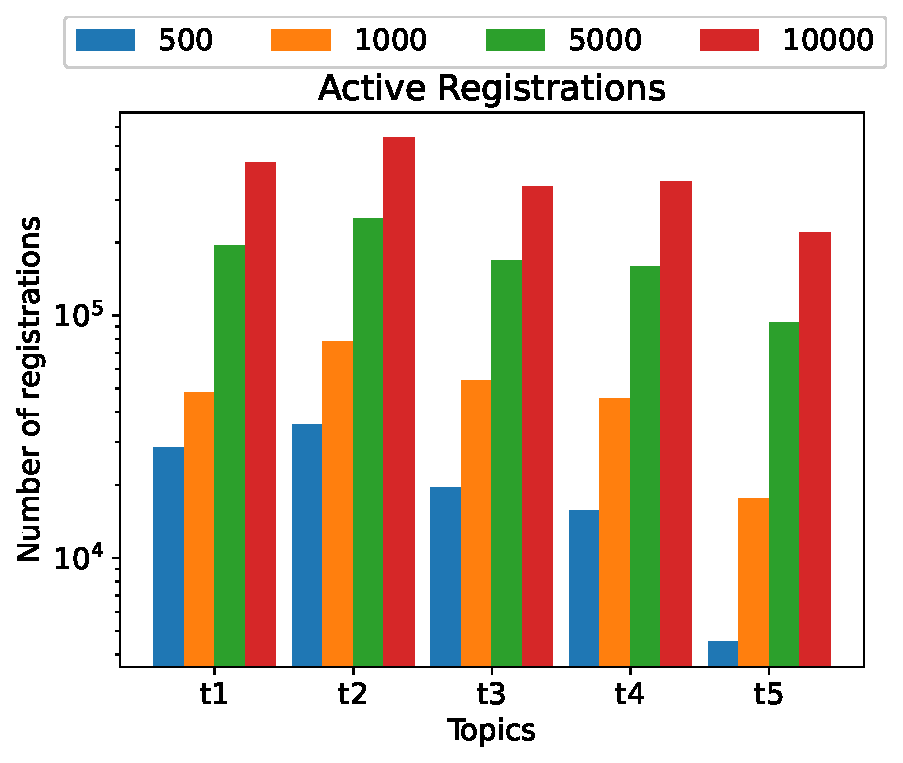
\includegraphics[width=0.225\textwidth]{img/eval/registration_origin.eps}
\label{fig:regs}
} 
\hspace{-0.25cm}
\subfigure[{Time to register}]{
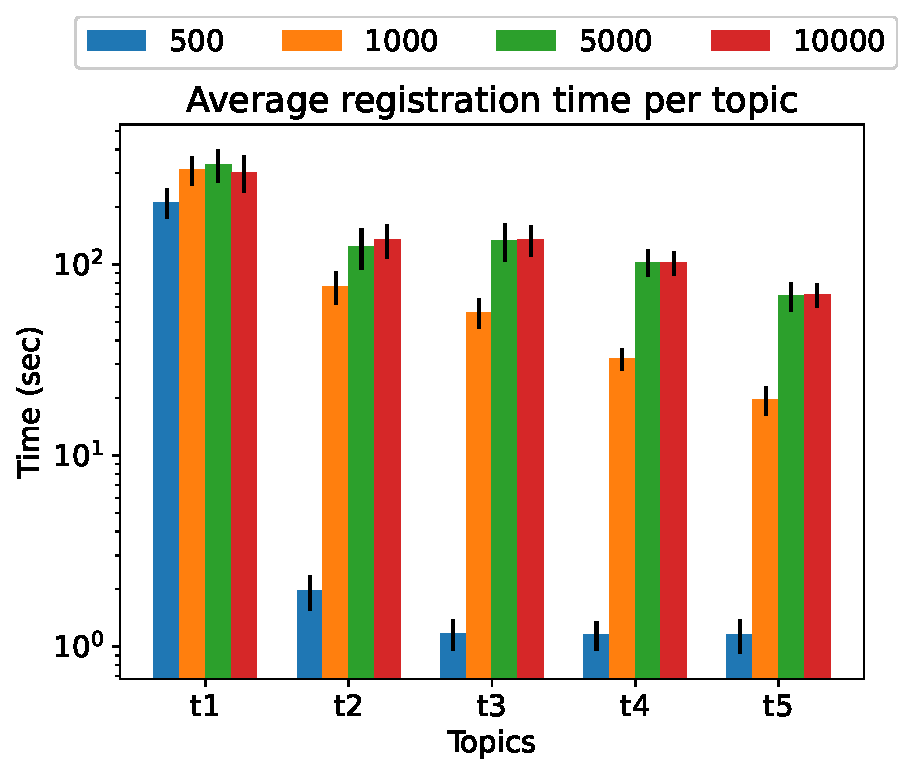
\includegraphics[width=0.225\textwidth]{img/eval/avg_time_register.eps}
\label{fig:time_reg}
}
 \caption{Ticket registrations} 
\label{fig:registrations}
\vspace{-0.15in}
\end{figure}   

%\begin{figure}[h!]
%\centering
%%\epsfig{file=imgs/eval/scen5.pdf, width=0.45\textwidth}
%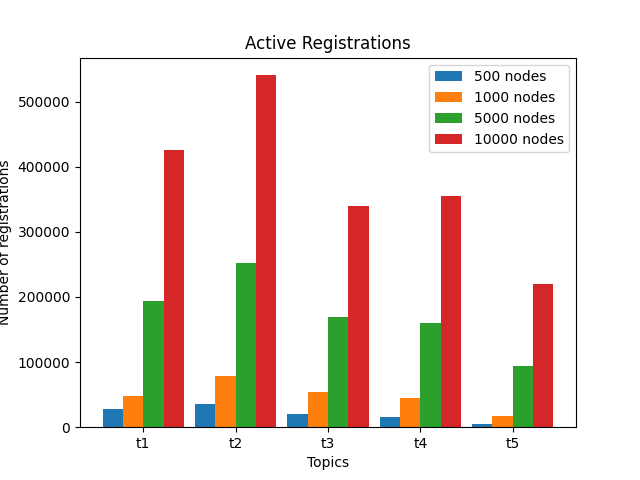
\includegraphics[width=0.225\textwidth]{img/eval/registration_origin.png}
%\caption{Registrations}
%\label{fig:regs}
%\vspace{-0.15in}
%\end{figure}

%\paragraph{\bf{Network load}:}
\subsubsection{Network load}

In Figure~\ref{fig:messages}~and~\ref{fig:msg_distr} we can observe the traffic load generated in the network.
In Figure~\ref{fig:messages} we observe most of the messages are ticket requests/replies, and the subsequent registration request/replies
after receiving a ticket from a node. 
This is caused by the fact that nodes are constantly registering dynamically. 
In Figure~\ref{fig:msg_distr} the messages received distribution. 
We can observe some nodes receive much more messages.
This is caused by the bucket node distribution, where nodes with identifiers close to topic hash ids receive more initial tickets requests because there are less.
However, we observe while the number of nodes in the network is increased 20 times,  the  maximum number of messages received by some nodes does not increase in the same way,  only being twice the amount when comparing 500 with 10000 nodes,  ans with increases lower than 30\% when number of nodes are doubled.
Moreover,  we can also see the number of messages received does not exceed 10 times the average value of the messages received. 

Therefore, the system is able to scale without danger of overloading some of the nodes of the network.

\begin{figure}[!h]
\centering
\subfigure[{Number of messages}]{
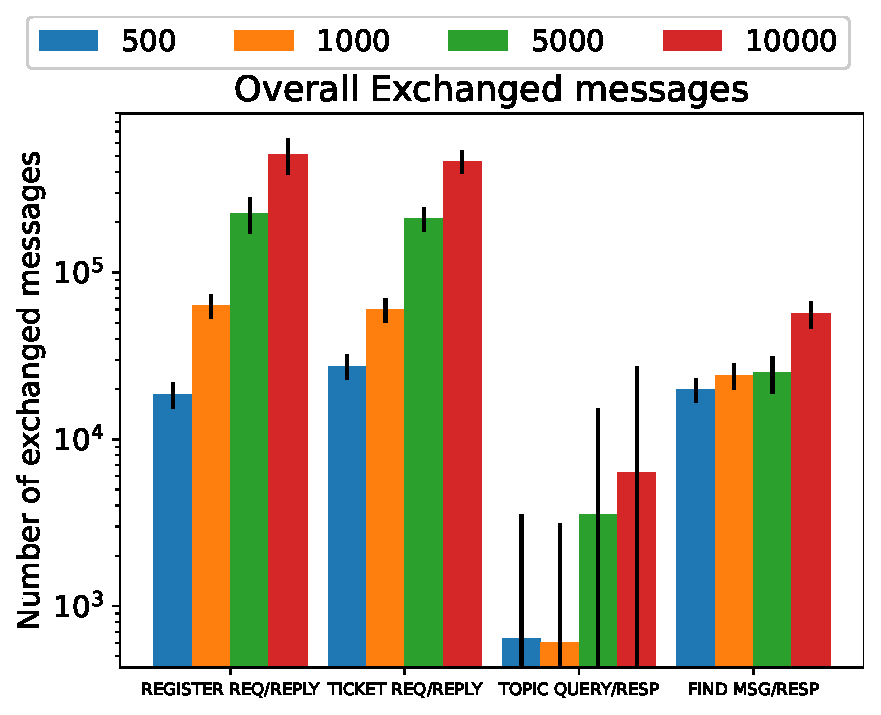
\includegraphics[width=0.225\textwidth]{img/eval/message_quantity.eps} 
\label{fig:messages}
} 
\hspace{-0.25cm}
\subfigure[{Message distribution}]{
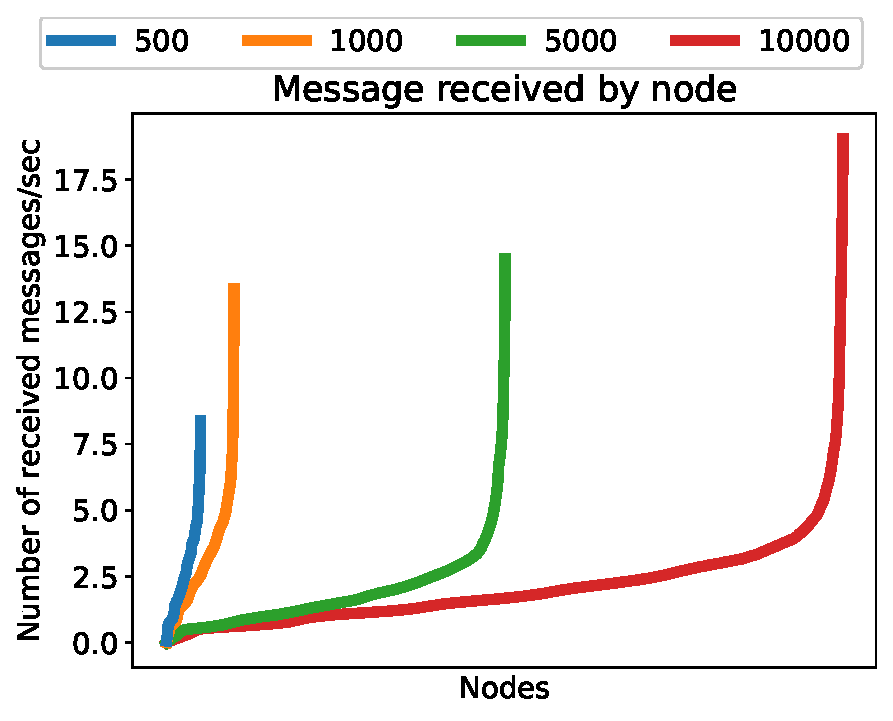
\includegraphics[width=0.225\textwidth]{img/eval/messages_received.eps} %\hspace{-1.5em}%
\label{fig:msg_distr}
}
 \caption{Traffic load} 
\label{fig:traffic}
\vspace{-0.15in}
\end{figure}   

\subsubsection{Discovery and lookup performance}

%\paragraph{\bf{Discovery performance}:}

In Figure~\ref{fig:reg_disc} and \ref{fig:timedisc} we can observe how nodes are discovered within the network.
In Figure~\ref{fig:reg_disc} we observe the percentage of the nodes in the network that are discovered and how often are discovered.
Each node in the network is represented by a circle, and the size of the cirle represents the relative frequency of discoveries compared with other nodes in the network.
We can observe that for all topics the percentage of nodes discovered in the network is very close to 100\%. This means almost all nodes in the network are able to be discovered by other nodes. The number of dicovered nodes is not 100\% because of the existence of turbulence (there are some nodes just joined the network and there has not been enough time yet to be discovered). In case there are a low number of nodes for a specific topic (e.g. t5 with 500 nodes network) the 100\% is reached.
We can also observe Figure~\ref{fig:reg_disc} that the discovery distribution is bounded to \hl{X} times between the most discovered and the least discovered.
We observe the dots size are very regular and despite being not completely equal the differences are not substantial. 
In Figure~\ref{fig:timedisc} we observe the time between a registration is completed and the first time the registration
is returned in a lookup.
By observing this we can see how difficult is for a node to be discovered once is able to place a registration. 
We see the average time is between 20 and 10 seconds in most of the cases, except for the least popular topic t5 which is around 50\% higher. 
We also observe the deviation is bounded at around 60 seconds, with equivalent different for t5.


\begin{figure}[!h]
\centering
\subfigure[{Registrant discovery distribution}]{
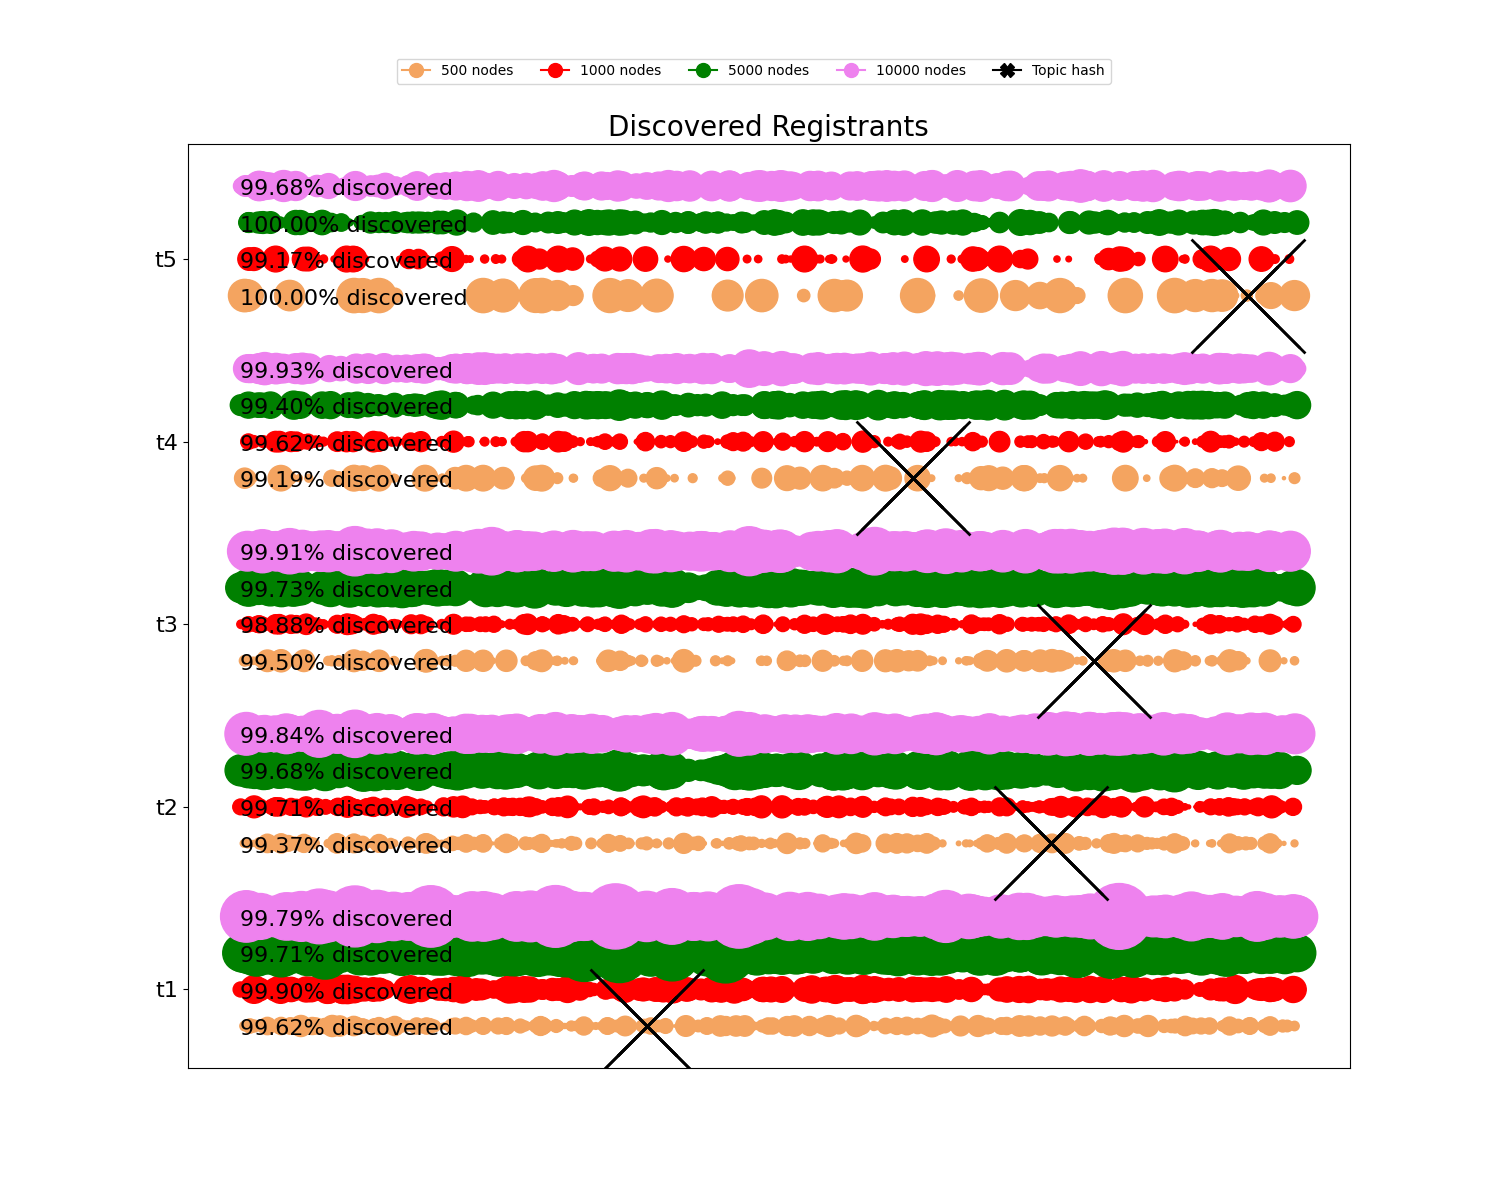
\includegraphics[width=0.225\textwidth]{img/eval/registrant_distribution.eps} 
\label{fig:reg_disc}
} 
\hspace{-0.25cm}
\subfigure[{Time between registration and first discovery}]{
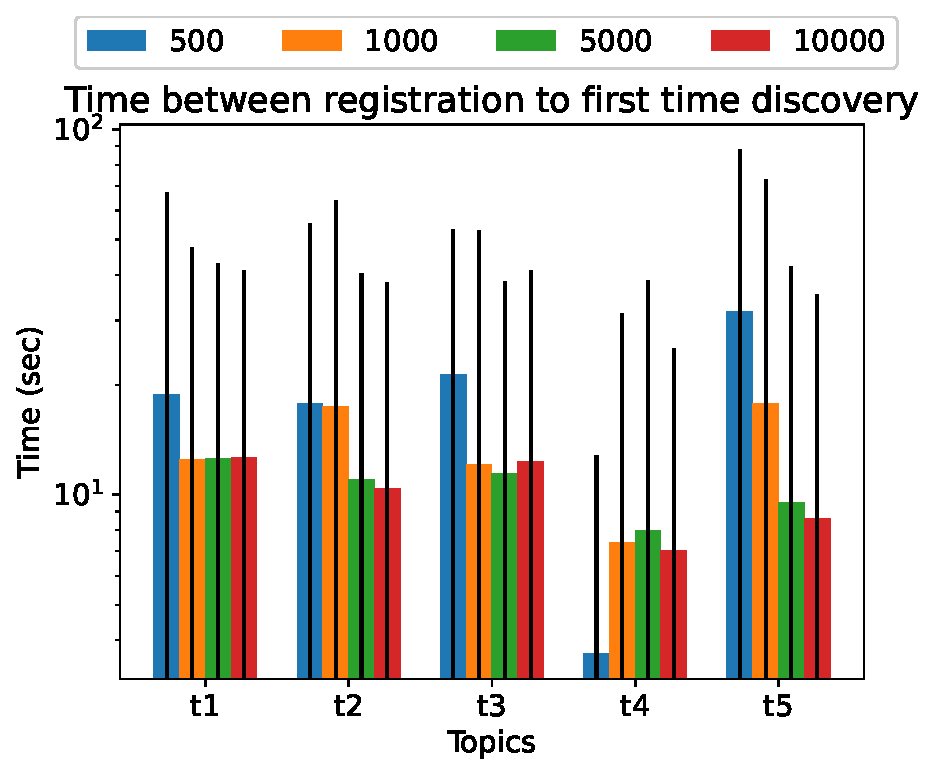
\includegraphics[width=0.225\textwidth]{img/eval/min_time_discovery.eps} %\hspace{-1.5em}%
\label{fig:timedisc}
}
 \caption{Discovery performance} 
\label{fig:discovery}
\vspace{-0.15in}
\end{figure}   


In Figure~\ref{fig:hopcount} we can observe the lookup performance of \sysname compared with Discv4 for a 5000 nodes simulation.
In the plot we show the average number of nodes discovered for each hop during a lookup per topic, taking into account that Discv4 cannot do per topic lookups,  so we discard received nodes that do not support the specific service.
In the figure we observe that for t1 the discovered nodes are higher when using Discv4, since all topics support t1 and any node discovered will be a valid node. 
However, as the popularity of the topic decreases it also does the lookup performance of Discv4,  since it is very difficult to find nodes for non-popular topics without supporting per topic lookups.
In this sense,  Discv5 lookup performance also decreases the performance with non-popular topics (simply because there are less nodes in the network) however this decrease is diminished.  Between t1 and t5 the lookup performance is decrease approximately to a 1/2th for Discv5, while when using Discv4 the lookup performance decreased to a less than a 1/10th.

%TODO add lookup description including mechanisms to avoid sybils.

\begin{figure}[h!]
\centering
%\epsfig{file=imgs/eval/scen5.pdf, width=0.45\textwidth}
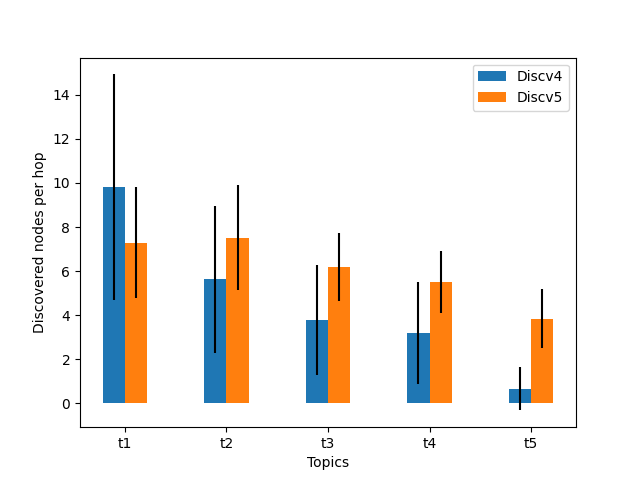
\includegraphics[width=0.35\textwidth]{img/eval/lookup_hopcount_discv4.png}
\caption{Lookup performance}
\label{fig:hopcount}
\vspace{-0.15in}
\end{figure}

\subsubsection{Sybil Attacks}

In the following we show the results of the performance evaluation of the discovery service under different sybil attacks.  The attacks that we evaluated in this section are of two types and are previously described in Section~\ref{sec:overview}. 
These attacks are eclipsing  and Denial-of-service (DoS) attacks.
Eclipsing attacks goal is to generate multiple fake identities within a topic to be able to eclipse existing nodes in the network.
Eclipsing a node imply all outbound and inbound connections are established to only sybil/fake nodes controlled by an attacker.
This allows the attacker to control the view of the network of the eclipsed node and can be used to co-opt a victim's mining power and use it to attack the blockchain's consensus algorithm.
DoS attacks instead is an attack meant to hamper the good performance or even to shut down the network, making it inaccessible to its intended users.  
In our case,  the goal of DoS attacks is to difficult or to block the discovery of nodes in the network and is specially important for topic with low popularity where finding all node in the network is very important.

In the implemented topic eclipsing attack,  malicious nodes are sybil nodes that cooperate in order to eclipse other valid nodes.
Malicious and valid nodes have the same amount of bandwidth resources and malicious nodes respond to topic lookup requests and find messages with only other malicious nodes.
Malicious nodes also act as evil 'registrants' trying to place as many registrations as possible by using bigger ticket size,  with malicious registrars attack,  where evil registrars replies with only malicious nodes when receiving a topic query.

We implemented and evaluated two kind of DoS attacks.  
The first attack consists in a topic spam attack where a big number of sybil identities generated try to register for non-existing random topics.
By registering for non-existing topics,  evil nodes try to harm valid topics registrations, overflowing topic tables.
The second DoS attack consists on generating sybil identities that keep without replying when receiving valid nodes ticket requests or return very long waiting times. 
This way an attacker can try to backlog valid nodes ticket registrations.

In Figures~\ref{fig:reg_eclipse},~\ref{fig:discoverytime_eclipse}~and~\ref{fig:lookup_eclipse} we show performance results under a
topic eclipsing attack.
We compare results for topic eclipsing attacks targeted to the most popular topic (t1) and attacks targeted to the least popular topic (t5). 
In the simulation there are 2000 nodes, all of them participating in t1 and only 218 participating in t5. 
In the simulations there are an additional 20\% (400 in total) malicious nodes that target the specific topic and the number of resources used in the attack (IP addresses) vary from 1 address to 50.

\begin{figure}[!h]
\centering
\subfigure[{Active registrations eclipse attack t1 attack}]{
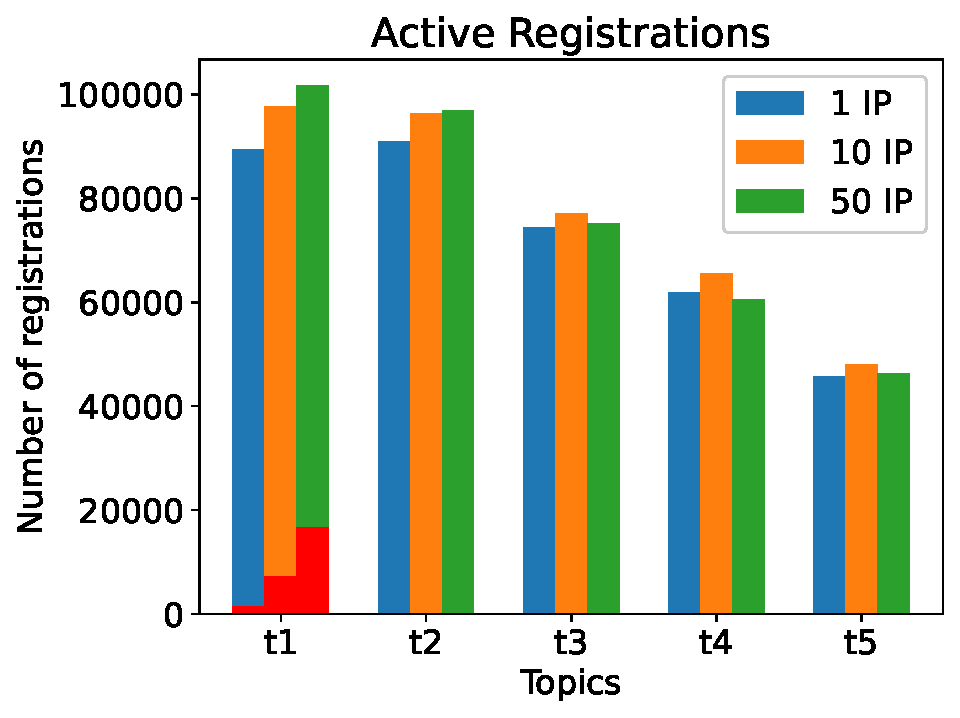
\includegraphics[width=0.22\textwidth]{img/eval/attack/registration_origin_t1.eps} 
\label{fig:reg_eclipse_t1}
} 
\hspace{-0.15cm}
\subfigure[{Active registrations eclipse attack t5 attack}]{
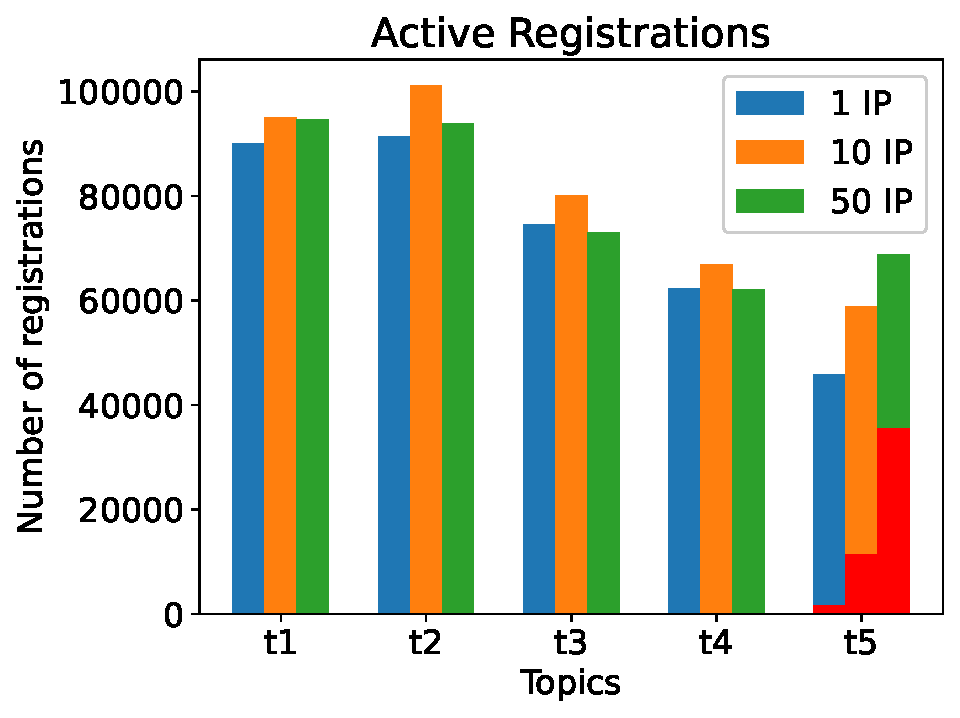
\includegraphics[width=0.22\textwidth]{img/eval/attack/registration_origin_t5.eps} %\hspace{-1.5em}%
\label{fig:reg_eclipse_t5}
}
 \caption{Active registrations under topic eclipsing attack} 
\label{fig:reg_eclipse}
\vspace{-0.15in}
\end{figure}   

In Figure~\ref{fig:reg_eclipse_t1} we observe the active registrations in the simulation per topic, for an eclipsing attack targeted to the most popular topic (t1), including active registrations of malicious nodes.
We can observe than even though the number of malicious nodes is equivalent to 20\%, the number of active registrations is lower than that. 
As expected, as the number of IP addresses used in the attack increaseas, the number of active registrations of malicious nodes also increase, since different malicious nodes with complete different IPs can not be diffierentiated from valid nodes.
For topic 5, the most vulnerable topic for being the least popular, we can observe a similar pattern of active registrations. 
However, we observe that despite malicious nodes being more (400 nodes) than valid nodes (218 nodes), active registrations of malicious nodes is kept lower than 30\% in all cases. Similarly to t1, the active registrations increase with the higher number of IPs used in the attack, since there is no way to a totally distributed attack without reusing IP addresses.


\begin{figure}[!h]
\centering
\subfigure[{Time between registration and first discovery t1 attack}]{
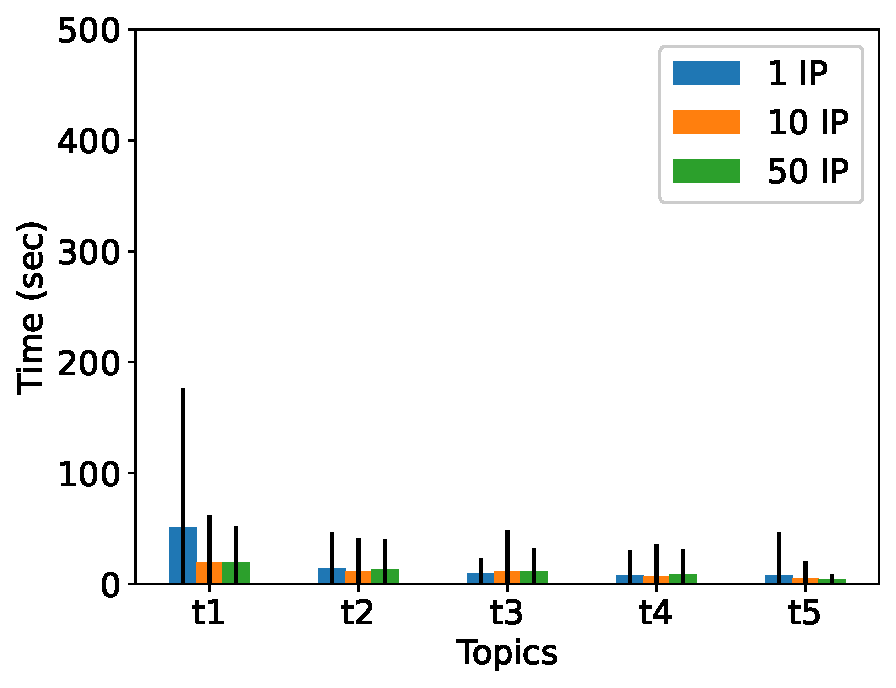
\includegraphics[width=0.225\textwidth]{img/eval/attack/min_time_discovery_t1.eps} 
\label{fig:discoverytime_eclipse_t1}
} 
\hspace{-0.16cm}
\subfigure[{Time between registration and first discovery t5 attack}]{
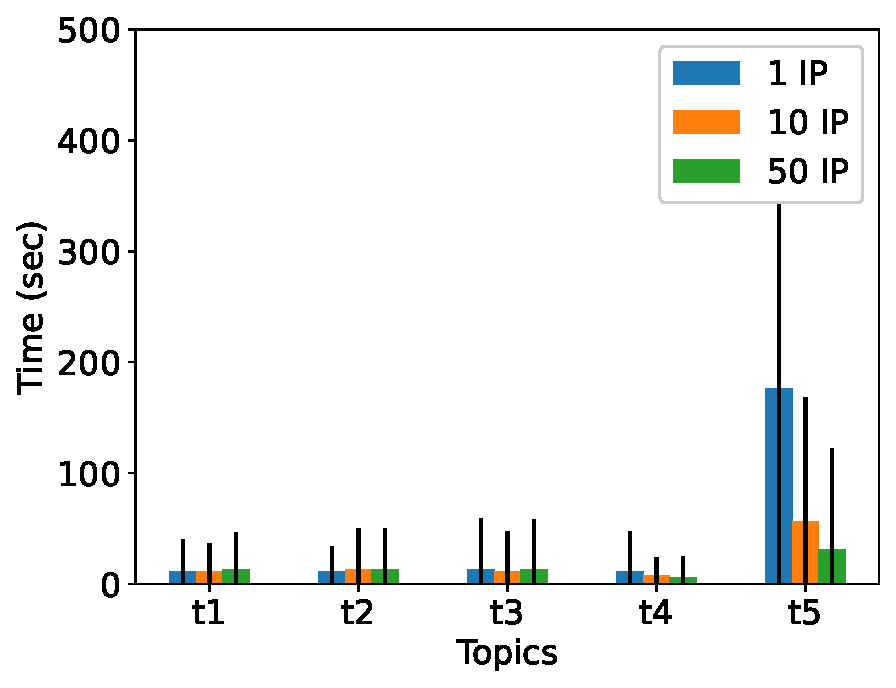
\includegraphics[width=0.225\textwidth]{img/eval/attack/min_time_discovery_t5.eps} %\hspace{-1.5em}%
\label{fig:discoverytime_eclipse_t5}
}
 \caption{Time between registration and first discovery under topic eclipsing attack} 
\label{fig:discoverytime_eclipse}
\vspace{-0.15in}
\end{figure}   

In Figure~\ref{fig:discoverytime_eclipse} we observe the average time between a node registers for a topic successfully and the node is discovered for the first time from the placed registration.
We can observe that when a topic is under attack the time required for first time discovery increases. 
This is caused by the fact that there are much more registrations in the topic caused by the attack and also that malicious nodes discovery time is higher due to the difficulty to place registrations in nodes close to the topic hash.  
We can observe that when using more IP addresses in the attack the time required to discover a node is reduced because malicious nodes are more discovered.

\begin{figure}[!h]
\centering
\subfigure[{Lookup hopcount eclipse attack t1}]{
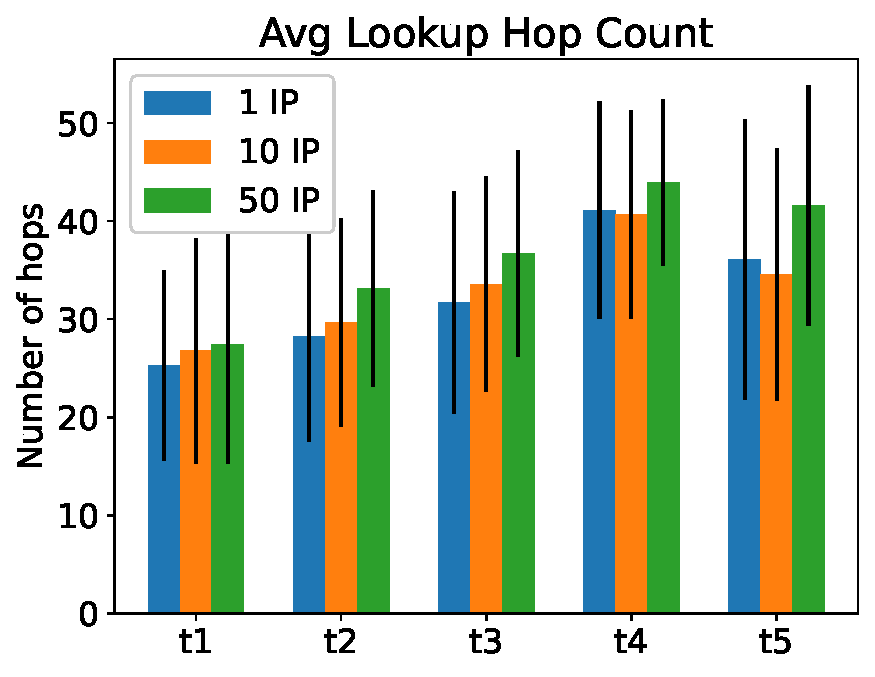
\includegraphics[width=0.225\textwidth]{img/eval/attack/lookup_hopcount_t1.eps} 
\label{fig:lookup_eclipse_t1}
} 
\hspace{-0.16cm}
\subfigure[{Lookup hopcount eclipse attack t5}]{
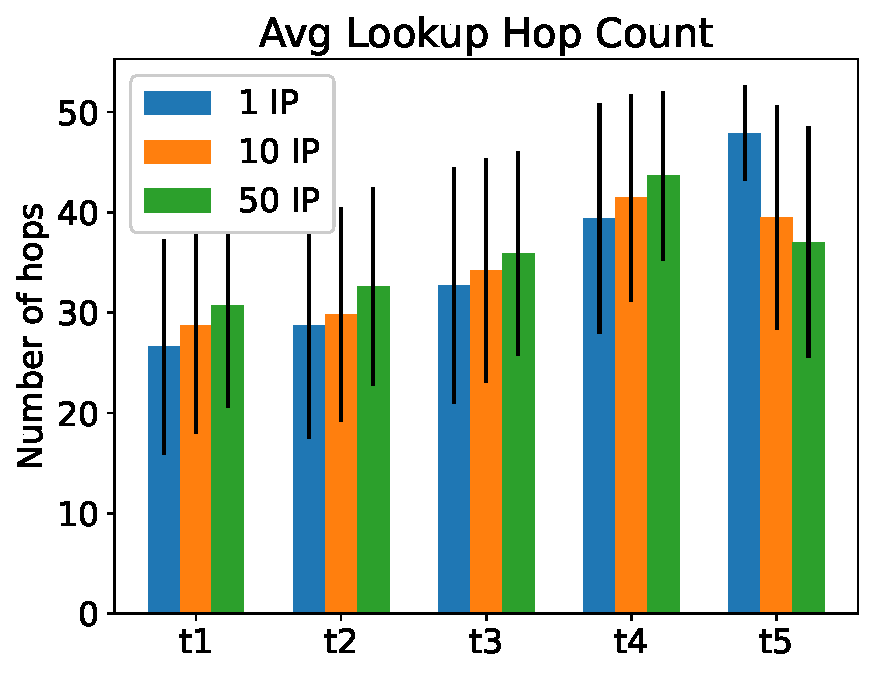
\includegraphics[width=0.225\textwidth]{img/eval/attack/lookup_hopcount_t5.eps} %\hspace{-1.5em}%
\label{fig:lookup_eclipse_t5}
}
 \caption{Lookup hopcount under topic eclipsing attack} 
\label{fig:lookup_eclipse}
\vspace{-0.15in}
\end{figure}   

\sergi{redo fig14 and fig15 figures increasing font and using eps}

In Figure~\ref{fig:lookup_eclipse} we observe the lookup hopcount in the simulation per topic,  for an eclipsing attack targeted to the most popular topic (t1) and the least popular topic (t5).
We observe that despite receiving an attack targeted at a specific topic,  the lookup performance in the network is not substantially affected by the attack.

In Figure~\ref{fig:perf_spam} we observe the performance of the topic discovery system under  the topic spam attack.
\sergi{TODO: add no sybil in the graph}
In Figure~\ref{fig:active_regs_spam} we observe the average active registrations per topic increasing the number of IP addresses used by sybil identities performing the attack.  
We observe that the number of active registrations per topic are decreased under the topic spam attack being topic 1 the most affected.
However, by observing Figure~\ref{fig:hopcount_spam} we see he lookup performance is not affected and therefore there is no substantial impact of the attack in the discovery performance of the network, concluding the system is resistant to topic spam attacks.
In Figure~\ref{fig:time_register_spam} we observe the average time required for registering for a topic,  increasing the number of Ip addresses used by sybil identities performing the attack.  
We observe again it seems there is no substantial impact of the attack to the time required to register for each topic

\sergi{add spam storage used?}

\begin{figure*}[!h]
\centering
\subfigure[{Active registrations under topic spam attack}]{
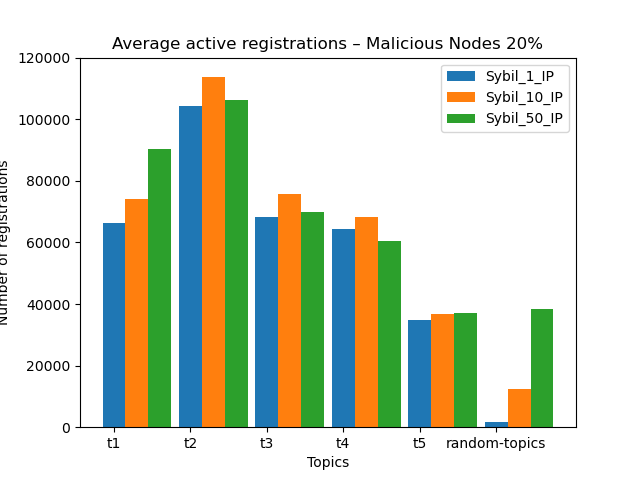
\includegraphics[width=0.275\textwidth]{img/eval/attack/registration_origin_spam.png} 
\label{fig:active_regs_spam}
} 
\hspace{-0.16cm}
\subfigure[{Time to register under topic spam attack}]{
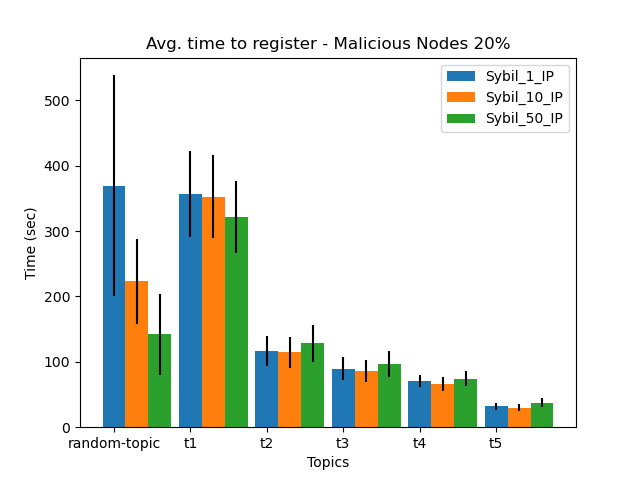
\includegraphics[width=0.275\textwidth]{img/eval/attack/avg_time_register_spam.png} %\hspace{-1.5em}%
\label{fig:time_register_spam}
}
\hspace{-0.15in}
\subfigure[{Lookup hop count topic spam attack}]{
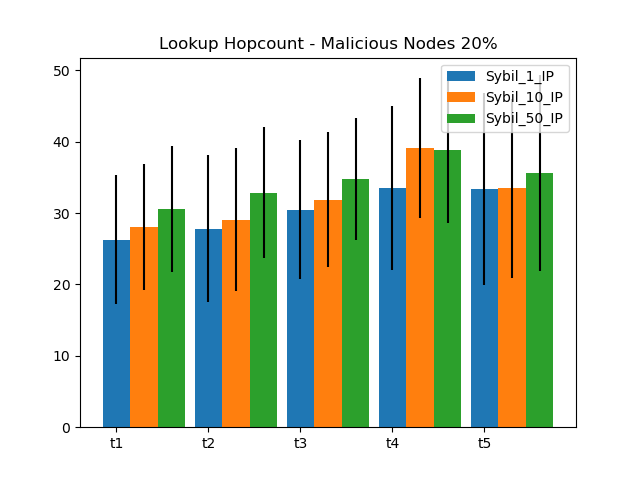
\includegraphics[width=0.275\textwidth]{img/eval/attack/lookup_hopcount_spam.png} %\hspace{-1.5em}%
\label{fig:hopcount_spam}
}
\caption{Performance evaluation topic spam attack} 
\label{fig:perf_spam}
\vspace{-0.15in}
\end{figure*}   

In Figure~\ref{fig:perf_dos} we observe the performance of the topic discovery system under the dos attack where registrars do not respond to advertisers trying to block active registrations.
In Figure~\ref{fig:active_regs_dos} we observe the average active registrations per topic increasing the number of sybil identites from 5\% to 20\% of the nodes in the network.
We observe that the number of registrations are affected by attackers,  being more affected for very popular topics,  but less affected low popularity topics.  However in none of the cases malicious nodes are able to block the active registrations and the reduction of the performance is lower than the number of sybils used.
In Figure~\ref{fig:time_register_dos} we observe the average time required for registering for a topic,  increasing the number of sybil identites from 5\% to 20\% of the nodes in the network.
We observe in this case it seems there is no substantial impact of the attack to the time required to register for each topic
In Figure~\ref{fig:time_discovery_dos} we observe the average time between an advertiser place a registration in a registrar and another node discovers it through the registrar,  increases the number sybils again.
We also observe there is no substantial impact of the attack, concluding the system is resistant to DoS attacks.

\begin{figure*}[!h]
\centering
\subfigure[{Active registrations under DoS attack}]{
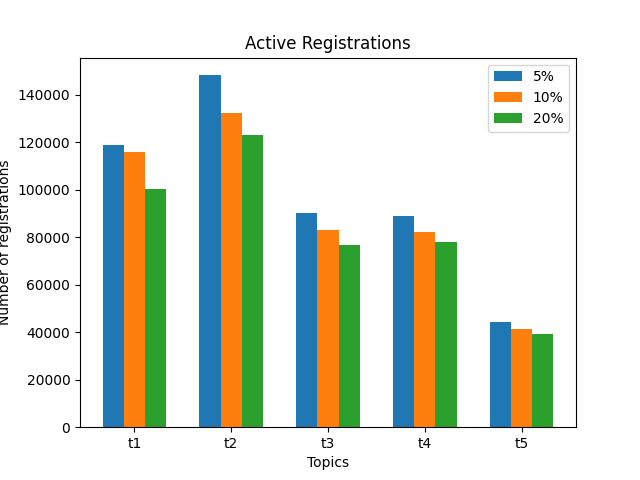
\includegraphics[width=0.275\textwidth]{img/eval/attack/registration_origin_dos.png} 
\label{fig:active_regs_dos}
} 
\hspace{-0.16cm}
\subfigure[{Time to register under DoS attack}]{
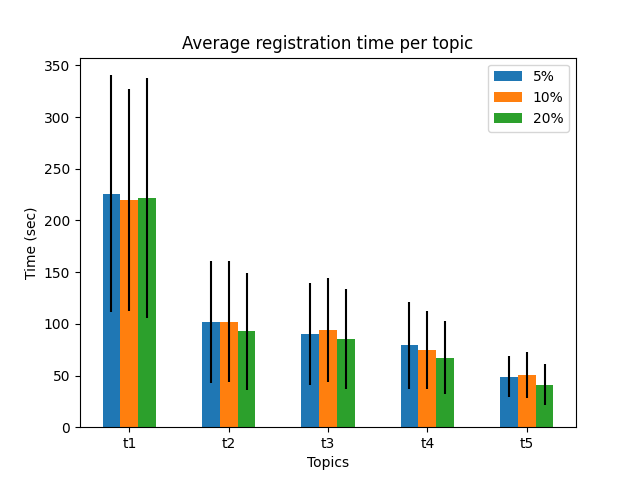
\includegraphics[width=0.275\textwidth]{img/eval/attack/avg_time_register_dos.png} %\hspace{-1.5em}%
\label{fig:time_register_dos}
}
\label{fig:discovery_dos}
\hspace{-0.15in}
\subfigure[{Time to first discovery under DoS attack}]{
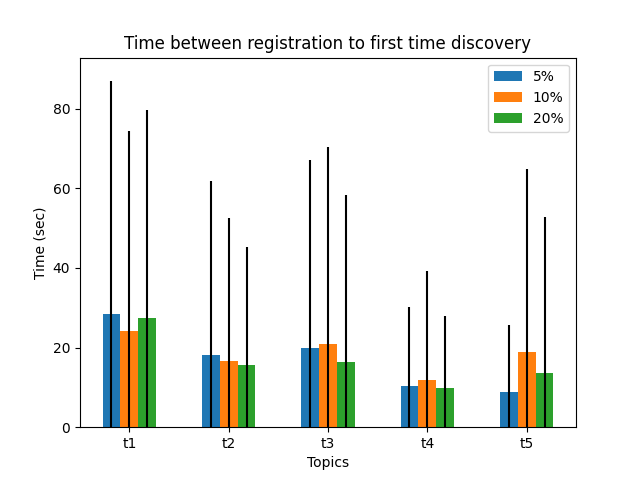
\includegraphics[width=0.275\textwidth]{img/eval/attack/min_time_discovery_dos.png} %\hspace{-1.5em}%
\label{fig:time_discovery_dos}
}
\label{fig:perf_dos}
\caption{Performance evaluation no-response DoS attack} 
\vspace{-0.15in}
\end{figure*}   


%\subsection{Testbed evaluation}
%
%"Geth"~\cite{go-ethereum} performance evaluation: \hl{TBC}.


%!TEX root = ../main.tex
%=========================================================

\section{Related Work}
\label{sec:related}

\er{Maybe discuss the byzantine-resilient peer sampling system Brahms, that also uses a blocking mechanism when more than a threshold number of view updates (pushes) are received in a certain amount of time (not sure if this is overall or for a specific node though)~\cite{}}

There exists several protocols aimed at discovery devices providing network services for local area networks.
For instance, the Simple Service Discovery Protocol (SSDP)~\hl{missing ref},  basis of the discovery protocol of Universal Plug and Play (UPnP)~\hl{missing ref},  or the DNS-based service discovery,  are used to advertise services that other devices provide,  such as printers,  webcams,  HTTPS servers, and other mobile devices,  usually using multicasting or broadcasting techniques.
However for service discovery in Internet-wide environments, since it is not possible to broadcast,
centralized setups are commonly used to provide service discovery with good performance.
UDDI~\hl{missing ref} has been recognized as the most popular discovery mechanism for
Web services.

But when focusing on decentralized architectures,  service discovery has been addressed from different perspectives. 
Most of the solutions use Distributed Hash Table (DHT) based protocols using key-based routing to discover other peers. 
CAN, Chord,  Pastry or Kademlia,  are examples of DHT protocols where all the nodes self-organize themselves into overlay networks. 
DHT-based solutions offer fault-tolerant,  scalable and efficient ways of finding nodes in large-scale networks.
However,  directly applying DHT for service discovery  present some drawbacks.
The main one is the difficulty in guaranteeing the availability of published service descriptions.
Usually,  DHT-based systems often distribute descriptions of functionally equivalent services to the same successor node,  as they have the same or similar hashing values. 
If such a node fails, a service consumer will not be able to discover any of these services. 
There are existing approaches that solve the issue. 
For instance,  Chord4S~\cite{chord4s} enhances Chord protocol by distributing service descriptions to different successor nodes. 
In case one node fails, a service consumer is still able to find functionally equivalent services that are stored at other successor nodes.

Another solution for service discovery on peer-to-peer overlay networks could be the use of topic-based pub/sub systems. 
These exists some solutions,  such as~\cite{scribe,poldercast,banno2015},  that uses DHT-based systems to multicast data to subscribers.
Similarly,  TERA~\cite{baldoni2007tera} uses topic-based pub/sub system
but using gossip protocols and self organization.  
%TERA provides a good balance between bandwidth consumption and performance guarantees. 
Similar solutions could be use to announce nodes that offer a certain service.
However,  those solutions rely on the use of rendezvous points for publishing the data,  which adds a single point of failure to the network.
Moreover,  continuous multicast of data to nodes subscribed for a service adds overhead to the network.
However,  all these solutions have not been designed with Sybil-resistance in mind and it requires that all nodes be trusted.

%"Centralized and distributed protocols for tracker-based dynamic swarm management"~\cite{dan2012centralized}


Another possible solution for service discovery in blockchain platforms is to incorporate a service discovery component to the blockchain. 
In~\cite{manevich2019endorsement}, a new service discovery component is presented for  Hyperledger Fabric (HLF),  a permissioned blockchain platform.
The service discovery component provides APIs that allow the client application to dynamically discover the configuration details of the endorsement policies and chaincode it needs to use.
However, since HLF is a smaller scale private blockchain it does not require large-scale service discovery as ours and it does not need to prevent this service discovery feature from attackers.

%"Endorsement in Hyperledger Fabric via service discovery"~\cite{manevich2019endorsement}: allows Hyperledger Fabric client to locate available services (chaincodes) using an API since HLF version 1.2. Before the set of services (chaincodes) was hardcoded at the client and server side. 
Similalry,  in~\cite{farmer2021decentralized} the authors propose decentralized identifiers for peer-to-peer service discovery.
%"Decentralized identifiers for peer-to-peer service discovery"~\cite{farmer2021decentralized}:
Besides the service discovery feature in Ethereum itself, some applications build service discovery over Ethereum, as in this example of decentralized identifiers (there are tons of examples of web services using the blockchain to store and retrieve service representatives)~\cite{keizer2021flock}.

%"Under the Hood of the Ethereum Gossip Protocol"~\cite{kiffer2021under}: a study of Ethereum gossip protocol that I did not read yet.

%Ethna~\cite{wang2021ethna} seems also similar.




%\subsection{Eclipse attacks in Eth/p2p}

%Approaches to leverage security in DHT-based networks.

In the area of avoiding Sybil and derived eclipsing attacks in peer-to-peer networks several solutions and state-of-the-art can be found in the literature.
In~\cite{danezis2005sybil},  different strategies are devised to make DHTs resilient to malicious nodes trying to poison lookups,  by routing queries in a way that minimizes trust bottlenecks,  to minimize the amount of poisoned information that honest nodes receive from adversarial nodes.
In a similar way,  S/Kademlia~\cite{skad} propose new mechanisms to get resilience against common attacks by using parallel lookups over multiple disjoint paths,  limiting free nodeld generation with crypto puzzles and introducing a reliable sibling broadcast.

In ~\cite{cholez2010efficient},  the authors propose  a statistical approach to detect a particular type of Sybil attack in  Kademlia DHT,  where Sybil peers strategically choose IDs that are close to a target ID in the DHT ID space.
The authors found that the expected the ID distribution of the closest nodes returned in the search results for target IDs follow a geometric distribution. Therefore, the divergence from geometric distribution of the node IDs in search results indicate existence of Sybil nodes in the results.  However, computing a divergence threshold is not straightforward and requires fine tuning to avoid false positives when detecting Sybil nodes.

In~\cite{marcus2018low}~and~\cite{henningsen2019eclipsing},  the authors present low-resource eclipsing attacks for the Ethereum P2P network.  
The attack ensures that the lookup-buffer used to initiate outbound connections is filled up with adversarial nodes by placing an adversarial node to each one of the DHT buckets, requiring only  2 IPs from distinct /24 subnets to be successful.
As a result of this paper, Geth v1.8 and v1.9 implemented new countermeasures,  such as  increasing number of connections, considering all nodes of the table during lookups,  or throttling the inbound connection attempt,  to reduce the chance of selecting an attacker-node .

%"Efficient DHT attack mitigation through peers' ID distribution"~\cite{cholez2010efficient} – This paper proposes a statistical approach to detect a particular type of Sybil attack in vanilla Kademlia DHT, where Sybil peers strategically choose IDs that are close to a target ID in the DHT ID space. If sufficient number of (i.e., typically 10 or more) Sybil peers are successfully placed closest to a target ID, then the Sybils could attract all or most of the search and registration requests for that ID because of their proximity to that target and launch attacks such as returning bogus search results. On the other hand, the normal behaviour of honest peers is to generate their IDs uniformly at random. Based on measurements on a DHT with only honest peers, the authors find that the expected the ID distribution of the closest nodes returned in the search results for target IDs follow a geometric distribution. Therefore, the divergence from geometric distribution of the node IDs in search results indicate existence of Sybil nodes in the results. Once divergence is detected, the IDs that contribute the most to the divergence are considered to be Sybils and are therefore omitted from the search results. However, computing a divergence threshold is not straightforward and requires fine tuning to avoid false positives when detecting Sybil nodes.


%S/Kademlia~\cite{skad}.
%"S-Kademlia"~\cite{pecori2016s}


Security lessons learned from literature:
\begin{itemize}
\item Assume that the underlying network layer does not provide any security properties to the overlay layer.
\item Importance of difficulty on generating random ids.
\item Nodes should not be capable of generating any id and duplicate ids should not be possible.  Ids should be linked to ip,  port or public key.
\item  Use of  parallel lookups over multiple disjoint paths to avoid querying only  adversarial nodes paths.
\item Importance of limiting IPs per bucket to require more resources to launch a sybil attack.
\item Avoid querying only nodes close to topic id / node id because adversarial nodes can strategically place nodes close to those ids.
\end{itemize}

%In "Eclipsing Ethereum Peers with False Friends"~\cite{henningsen2019eclipsing} - ,  the authors present  a false friends attack,  an eclipse attack applicable to Geth version v1.8.20.  The attack ensures that the lookup-buffer used to initiate outbound connections is filled up with adversarial nodes by placing an adversarial node to each one of the DHT buckets. 
%Since there is a limit that at most 2 nodes from the same /24 subnet can be included in the same bucket and at most 10 nodes from the same /24 can be in the whole table,  it requires  2 IPs from distinct /24 subnets to be successful,  and in contrast
%with previous attacks, it can be successfully mounted without
%assuming that the victim node reboots at some point, and can be completed in a matter of days.
%In response to the attack presented in the paper,  Geth version v1.9.0 implemented new countermeasures,  such as i) increasing number of connections from 25 to 50 ii) considering all nodes of the table during lookups, instead of only the bucket heads,  to reduce the chance
%of selection an attacker-node and iii) throttle the inbound connection attempts to limit the consecutive inbound connection attempts from the same IP to 30 seconds.

%"Low-Resource Eclipse Attacks on Ethereum's Peer-to-Peer Network."~\cite{marcus2018low} - 

"Sybil-resistant DHT routing"~\cite{danezis2005sybil} - they enhance standard DHT routing with information about the social network (by whom the nodes where introduced into the DHT). Based on that, they try to detect and avoid Sybils. Again, we don't have an introduction social network. 

\sergi{I haven't read these papers yet. To be included}
"A Sybil-proof one-hop DHT"~\cite{lesniewski2008sybil}

"Sybilinfer: Detecting sybil nodes using social networks."~\cite{danezis2009sybilinfer}
SybilInfer is an algorithm aimed at detecting Sybil attacks in social networks using e Bayesian inference approach.  It  labels which nodes are honest and which are dishonest with a degree of certainty. The decision is based on an analysis of social connections. However, it requires a social network that we do not have in our setup. 

"Whanau: A sybil-proof distributed hash table"~\cite{lesniewski2010whanau} - 


"Persea: a sybil-resistant social dht"~\cite{al2013persea} - 


"Design and evaluation of Persea, a Sybil-resistant DHT"~\cite{al2014design} - 

"Defending the sybil attack in p2p networks: Taxonomy, challenges, and a proposal for self-registration"~\cite{dinger2006defending}


"Quantitative analysis of the sybil attack and effective sybil resistance in peer-to-peer systems"~\cite{jetter2010quantitative}


GossipSub: Attack-Resilient Message Propagation in
the Filecoin and ETH2.0 Networks~\cite{gossipsub}


\section{Conclusions}
\label{sec:con}



%%!TEX root = ../main.tex
%=========================================================

\section{Notes}
Increase the blacklisting time to sth higher than ad\_lifetime

Introd why


Discovery - state that we do a fix betad non-



\subsection{Tasks}
Paper: 

\begin{itemize}
	\item Write abstract
    \item Complete intro
    \item Complete background
    \item Describe all the attacks we already considered (where?)
    \item complete related work
    \item complete missing references
    \item add python simulation results and scenario description in performance evaluation
    \item add security results  in performance evaluation
\end{itemize}

Other tasks:

\begin{itemize}
	\item Get past attack traces from Felix
    \item IP -> new system (done?)
\end{itemize}

\clearpage
% ========= references =========
\bibliographystyle{plain}
\bibliography{references}

\end{document}
